% 	This template is  MIT licensed.

% 	Basic file to demonstrate the usage of this LaTeX template.
% 	You can build your own paper/thesis on top of this file.
% 	Simply adjust the document class and all metadata and start working.
%
\documentclass[
	language=english, % set to english or german
	type=bachelor, % set to bachelor, master or seminar
]{isthesis}

% Graphics rendering using TikZ
% See: https://en.wikibooks.org/wiki/LaTeX/PGF/TikZ

\usepackage{tikz}
% \usepackage{graphicx}
% \usepackage{caption}
% Include required TikZ libraries here, some exemplary libraries are pre-included
\usetikzlibrary{calc}
\usetikzlibrary{matrix}
\usetikzlibrary{positioning}
\usetikzlibrary{shapes.geometric}
%Add your library here
\addbibresource{library.bib}

% Import acronyms
% \newacronym[longplural={<long plural>}, shortplural={<short plural>}]{<label>}{<short>}{<long>}
% 	label = is the unique identifier and sort key for the acronym, can be the same as <short>
%	short = is the abbreviation or acronym
%	short plural (optional) = is the plural of the abbreviation or acronym
%	long = is the long form of the acronym, this will appear in the list of abbreviations
%	long plural (optional) = is the long plural form of the abbreviation or acronym

\newacronym[shortplural={KMUen}, longplural={Kleine und Mittlere Unternehmen}]{kmu}{KMU}{Kleines und Mittleres Unternehmen}
\newacronym{CD}{CD}{Corporate Design}
\newacronym{SQL}{SQL}{Structured Query Language}
\newacronym{FAU}{FAU}{Friedrich-Alexander-Universit\"at Erlangen-N\"urnberg}
\newacronym{BPM}{BPM}{Business Process Management}
\newacronym{npm}{NPM}{Node Package Manager}
\newacronym{diss}{DISS}{Digital Industrial Service System}


% Import symbols
% Syntax: <Symbol> <Label> <Name>
% The symbols are sorted by their labels
\addsymboltolist{$\Pi$}{Pi}{Projection}
\addsymboltolist{$\Join$}{Join}{Natural Join}
\addsymboltolist{$\sigma$}{Selection}{Selection}


% Import custom commands
% If you want to define custom commands, please do so here
\DeclareUnicodeCharacter{03B1}{$\alpha $}
\DeclareUnicodeCharacter{03B2}{$\beta$}
\DeclareUnicodeCharacter{03B3}{$\gamma$}
\DeclareUnicodeCharacter{03B4}{$\delta$}
\DeclareUnicodeCharacter{03B6}{$\zeta $}
\DeclareUnicodeCharacter{03B7}{$\eta $}
\DeclareUnicodeCharacter{03B8}{$\theta $}
\DeclareUnicodeCharacter{03BA}{$\kappa $}
\DeclareUnicodeCharacter{03BB}{$\lambda $}
\DeclareUnicodeCharacter{03BC}{$\mu $}
\DeclareUnicodeCharacter{03BE}{$\xi $}
\DeclareUnicodeCharacter{03C0}{$\pi $}
\DeclareUnicodeCharacter{03C6}{$\phi $}
\DeclareUnicodeCharacter{03C9}{$\omega $}



% Document meta information
\isthesis{
    title={Development of a web-oriented code modeling the propagation of ultrashort pulses in optical fibre},
    author-name={Hernan Alberto Aguilera Abril}, % Separate multiple authors with commas
    author-email={hernan.aguilera@fau.de},
    %author-phone={+49 1776300853}, % Use international numbers format
    author-matriculation={Matrikelnummer: 22710623},
    % author-address={Erwin Rommel Str. 53},
    % author-zip={91058},
    author-city={Erlangen},
    principal-supervisor={Prof. Dr.-Ing. Bernhard Schmauss}, % This must be a professor
    associate-supervisor={Prof. Dr. Nicolas Joly}, % This is your main supervisor, i.e., a post doc or doctoral student
    tutor-supervisor={}, % If required, define an additional supervisor resp. tutor here
    group={Lehrstuhl für Hochfrequenztechnik},
    group-institute={Friedrich-Alexander University of Erlangen-Nuremberg},
    %studies={B.Sc. Elektrotechnik – Elektronik – Informationstechnik}, %your field of studies, i.e. Wirtschaftsinformatik or International Information Systems
    %
    %associate-group={}, % When the thesis is done in cooperation with another chair, add it here
    %associate-group-institute={}, % add cooperating institute or university here
    seminar={Photonik}, % The title of your seminar
    submission-date={2021-10-04} % The date you handed in your document: Format yyyy-mm-dd
    %primary-logo={}, % Uses the FAU logo by default
    %primary-logo-height={}, % Uses 16mm as default height
    %secondary-logo={}, % Logo of the secondary institution (cooperating chair/university), USES Faculty logo by default
    %secondary-logo-height={} % Uses 16mm as default height
}


\begin{document}
    % Title page
    \newcounter{savepage}
    \maketitle

	% Quote
    % You can put an optional quote page in front of your content
    %   \quotepage[author={Arthur C. Clarke}]{
    %   	        Any sufficiently advanced technology is indistinguishable from magic.
    %   }
    
    % Table of contents
    \tableofcontents

    % List of figures (if you have figures)
    \listoffigures
    
    % List of tables (if you have tables)
    %\listoftables
    
    % List of listings (if you have listings)
	%\lstlistoflistings

    % List of abbreviations (if you use acronyms)
    \listofabbreviations
    
    % List of symbols (if you use symbols)
    %\listofsymbols
	
	% Abstract
	%
	% Comment out this part, if you don't require an abstract
	\begin{abstract}
	    % Add your abstract here:
		\lipsum[1]
		%la  importancia de las comunicaciones con fibra optica ha venido aumentando en los últimos anos debido a su alta quality (bajas pérdidas y hablar mierda de eso), así mismo, el estudio de las comunicaciones opticas ha venido en aumento, por ello, es importante que los estudiantes entiendan a profundidad los conceptos que encierran a las comunicaciones ópticas, ya sea desde la práctica o desde un punto de vista físico. Diversas herramientas pueden ser utilizadas en el aprendizaje de los estudiantes, entre ellas estan las aplicaciones web, las cuales, debido a su fácil acceso y amplio desarrollo, permiten a los estudiantes acceder a la información que requieran cuando la requieran. Se desarrolló entonces una aplicación web implementando un código en python, capaz de solucionar las diversas ecuaciones presentadas en el libro AGRAVAL, displaying los diversos fenómenos que afectan las comunicaciones opticas no lineares, tales como la dispersion y las no linearidades como es el caso del SPM. Primero fueron tratados los efectos por separado (en un principio la dispersion y luego las no linearidades), luego, con la ayuda del SSFM para la solución de la NLSE, se pudo ver el efecto de ambos fenómenos actuando al mismo tiempo en la fibra optica. Finalmente se deploy una web app capaz de solucionar de forma rápida la NLSE con el cambio de ciertos parámetros y presentar los cambios / broadening tanto en el tiempo como en la frecuencia dependiendo el caso. 
	\end{abstract}
	
	% storing the last pagenumber
    \setcounter{savepage}{\value{page}}
    
    
    % Content
    \begin{content}
        % Add your content files:
		\chapter{Introduction}
Objective:
Develop a tool for the future students who will study nonlinear optics in fibres so that they can appreciate more easily the different physical processes happening to a short pulse propagating in a dispersive nonlinear medium. These include the influence of the dispersion (second and third order), the self-phase modulation, the emission of dispersive wave, the soliton dynamics. Eventually, the code will be released as a web-interface for the future students to directly modify the physical parameters of the pulse, but also of the fibre.**



This \LaTeX \- template has been developed by the University of M\"unster and adapted by the Chair of Digital Industrial Service Systems at the \gls{FAU} to match the \gls{FAU} \gls{CD}. The file \path{main.tex} is the master file.

It was originally built by  Jan Betzing and Dominik Lekse and draws from the DBIS template by Till Haselmann and Florian Stahl, as well as from the IS template by Stephan Dlugosz. The adaption to FAU was done by Matthias Stierle. Currently, Sebastian Dunzer maintains the template.

This document is work-in-progress and provides instructions on how to use the template. It does not give advices on scientific writing.

Please feel free to contribute to this template.

\paragraph{TODO}
\begin{itemize}
	\item Configuration switch for having \textbackslash chapter\{\} begin on a new page
	\item Replace \texttt{kvoptions} with \texttt{pgfkeys}
\end{itemize}
		%\chapter{Literature review}

This chapter aims to review some of the existing theories about interactive learning and how to enhance the experience of the students. Some projects presented help to the construction and planning of the final product desired: a web-oriented code modeling the propagation of ultrashort pulses in optical fiber.

\section{Background: Constructivism and other theories of education}
\subsection{Constructivism}
Constructivism is a theory of cognition that proposes using unconventional instruction methods to fulfill the ever-active process of learning while not ignoring the idea that students are individuals who may perceive the learning environment in a different way than how the teachers intend to present it. Moreover, according to \cite{fosnot2013constructivism}, "the task of the educator is not to dispense knowledge but to provide students with opportunities and incentives to build it up;" that means adapting to the diverse forms of thinking instead of assuming that the students will acquire this knowledge just from the means already given.


\subsection{E-Learning}
The increasing quantity of online, partially online, or presential courses with strong online interactions strives to supply the necessity from a generation of students (with a strong influence of technology and social networks) to incorporate E-Learning in the teaching methods and the learning environments.  According to \cite{vltool}: "interactivity is a key feature of online education which helps attract and retain students in online classes," thus applying visual learning tools together with an online learning experience can develop engagement and motivation in the learning process in students. 

One can refer then to E-Learning as "the use of both software-based and online learning"  \cite{tabak} and, according to \cite{tabak}, \cite{munoz}, it has to be flexible, accessible, and intuitive. Hence factors like clear instructions, the relevance of the topics, the requirements to use its tools, and the difficulty to use them are crucial to implementing E-learning in different courses for different levels of education.

\section{Background: Interactive Learning tools}

Enhancing the students' learning experience regardless of the education level can be achieved using different interactive E-Learning tools, e.g., Web sites like Mathweb or mobile apps like I-MMAAPS. The interface of the interactive and personalizable content of these tools is essential to create a successful and effective tool \cite{vltool}. Therefore it should also be taken into account while creating an interactive E-Learning tool. Chapters 1 and 2 discuss how the interface was designed  and how a group of students perceived it.\textbf{ (give more details at the end of the project). }



\subsection{examples of Interactive Learning tools}
To know more about interactive learning is imperative to look at previous works and how they can contribute to the creation of new tools like the one discussed in this thesis.

\subsubsection{Mathweb}
The Hochschule Ruhr West has developed a website named \href{https://mathweb.de/}{"Mathweb"}   to support the students during the semester and preparation for the exams. According to surveys,  students underestimate the continuous study (during and after evaluations), among other problems related to learning strategies, that led to the endorsement of this Web amongst the students who, after the trial period, see it as a helpful tool and perceive a positive impact in their studies \cite{MathWeb}.

On this website are available a wide variety of examples, interactive demonstrations with graphics, explanations, exercises, and the option to check if the solution given by the user is correct. The themes included going from simple mathematical operations to more complex topics like derivatives are available for everyone, even though the test course cannot be accessed signed in as a guest.

\subsubsection{I-IMAPPS}

I-IMAPPS is an application created at the Universiti Teknologi MARA Sarawak in Malaysia and aimed to promote the learning of the indigenous Iban language using situations immerse in possible environments where its use is necessary. The researchers worked based on constructivism and the premise that mobile learning is an alternative to study a language if the people do not have the time for intensive or immersive lessons. 


To develop and structure this app, they followed the ADDIE Model, which consists of five aspects: 

\begin{enumerate}
    \item Analysis: gathering and selecting the information, phrases, and vocabulary of the Iban language; investigation on the availability (if there are existing apps created for this purpose, which is not the case) and focus on the learning objectives of the mobile app.
    \item Design: description of the message to send and the user interaction with the content, layout, and storyboard design focused on the cultural aspects of this language. The content framework comprehends the resources (multimedia elements like text, audio animations, etc.), learning theories allowing the user to work autonomously, and interactivity.
    
    \item Development: the researchers used Flash for the animations, Photoshop CS5  for the illustrations, and Corona SDK for software engineering. 

    
    \item Implementation.
    
    \item Evaluation: 30 non-native speakers tested the I-MMAPPS prototypes, did a test of the new knowledge obtained, and gave feedback on the experience using them.
    
\end{enumerate}

The conclusion of this research points that this app helps developing interest and assists non-native speakers at the early stages of learning this language. Further work needs to be done to improve the app's features \cite{CHACHIL2015267}. 



\subsubsection{Control courses}
Björn Wittenmark, Helena Haglund, and Mikael Johansson at Lund Institute of Technology used interactive learning and dynamic pictures to aid the students while learning abstract parts of the theory in control courses. The goal was not just to have students with a solid theoretical understanding of the topics but also to have high engineering capabilities; this relies on the good connection of the theory by improving the comprehension of the students and the practical aspect of the problems presented. One way to achieve this is with material available "anywhere and anytime" using the web and Matlab and Simulink for the computations. 

They implemented dynamic pictures where the user can see the effect of, e.g., changing a parameter in continuous-time poles and zeroes plots without typing commands. Drags, dropdowns, text input slots, and buttons enhance the graphical interface of the CCSDEMO. This tool makes active learning possible covering topics like robustness, tuning of PID-controllers, observability, among other subjects of the 13 available modules. They highlight the idea that it is meaningful to design the interface carefully to allow an intuitive use avoiding the need to read a manual and contributing to the utilization without supervision.

In conclusion, dynamic pictures improve the courses giving the students more tools than just pre-canned video or static data and illustrations, motivating the students who responded encouragingly \cite{IEEEcontrol}.



\subsubsection{Fiber-Modes App}

As previous work



		\chapter{Theoretical Framework}

This chapter reviews the actual state and the basis of the e-learning, as well as the theoretical base to model ultrashort-pulse propagation in fibers. Spectral and time broadening are fundamental aspects of nonlinear fiber optics. Understanding their basis and how they affect the propagation of an electromagnetic wave is an essential factor to both develop the code and test its effectiveness. Providing an overview of the equations describing the light propagation in a dispersive, nonlinear medium gives the principles to see what is solved with the back-end code at further stages in this thesis project.




\section{Background: Constructivism and other theories of education}
This section aims to review some of the existing theories about interactive learning and how to enhance the experience of the students. Some projects presented help to the construction and planning of the final product desired: a web-oriented code modeling the propagation of ultrashort pulses in optical fiber.



\subsection{Constructivism}
Constructivism is a theory of cognition that proposes using unconventional instruction methods to fulfill the ever-active process of learning, this while not ignoring the idea that students are individuals who may perceive the learning environment in a different way than how the teachers intend to present it. Moreover, according to \cite{fosnot2013constructivism}, "the task of the educator is not to dispense knowledge but to provide students with opportunities and incentives to build it up;" that means adapting to the diverse forms of thinking, instead of assuming that the students will acquire this knowledge just from the means already given to them.


\subsection{E-Learning}
The increasing quantity of online, partially online, or presential courses with strong online interactions strives to supply the necessity from a generation of students (with a strong influence of technology and social networks) to incorporate E-Learning in the teaching methods and the learning environments.  According to \cite{vltool}: "interactivity is a key feature of online education which helps attract and retain students in online classes," thus applying visual learning tools together with an online learning experience can develop engagement and motivation in the learning process in students. 

One can refer then to E-Learning as "the use of both software-based and online learning"  \cite{tabak} and, according to \cite{tabak}, \cite{munoz}, it has to be flexible, accessible, and intuitive. Hence factors like clear instructions, the relevance of the topics, the requirements to use its tools, and the difficulty to use them are crucial to implementing E-learning in different courses for different levels of education.

\section{Background: Interactive Learning tools}

Enhancing the students' learning experience regardless of the education level can be achieved using different interactive E-Learning tools, e.g., Web sites like Mathweb or mobile apps like I-MMAAPS. The interface of the interactive and personalizable content of these tools is essential to create a successful and effective tool \cite{vltool}. Therefore it should also be taken into account while creating an interactive E-Learning tool. Chapters 1 and 2 discuss how the interface was designed  and how a group of students perceived it.\textbf{ (give more details at the end of the project). }



\subsection{examples of Interactive Learning tools}
To know more about interactive learning is imperative to look at previous works and how they can contribute to the creation of new tools like the one discussed in this thesis.

\subsubsection{Mathweb}
The Hochschule Ruhr West has developed a website named \href{https://mathweb.de/}{"Mathweb"}   to support the students during the semester and preparation for the exams. According to surveys,  students underestimate the continuous study (during and after evaluations), among other problems related to learning strategies, that led to the endorsement of this Web amongst the students who, after the trial period, see it as a helpful tool and perceive a positive impact in their studies \cite{MathWeb}.

On this website are available a wide variety of examples, interactive demonstrations with graphics, explanations, exercises, and the option to check if the solution given by the user is correct. The themes included going from simple mathematical operations to more complex topics like derivatives are available for everyone, even though the test course cannot be accessed signed in as a guest.

\subsubsection{I-IMAPPS}

I-IMAPPS is an application created at the Universiti Teknologi MARA Sarawak in Malaysia and aimed to promote the learning of the indigenous Iban language using situations immerse in possible environments where its use is necessary. The researchers worked based on constructivism and the premise that mobile learning is an alternative to study a language if the people do not have the time for intensive or immersive lessons. 


To develop and structure this app, they followed the ADDIE Model, which consists of five aspects: 

\begin{enumerate}
    \item Analysis: gathering and selecting the information, phrases, and vocabulary of the Iban language; investigation on the availability (if there are existing apps created for this purpose, which is not the case) and focus on the learning objectives of the mobile app.
    \item Design: description of the message to send and the user interaction with the content, layout, and storyboard design focused on the cultural aspects of this language. The content framework comprehends the resources (multimedia elements like text, audio animations, etc.), learning theories allowing the user to work autonomously, and interactivity.
    
    \item Development: the researchers used Flash for the animations, Photoshop CS5  for the illustrations, and Corona SDK for software engineering. 

    
    \item Implementation.
    
    \item Evaluation: 30 non-native speakers tested the I-MMAPPS prototypes, did a test of the new knowledge obtained, and gave feedback on the experience using them.
    
\end{enumerate}

The conclusion of this research points that this app helps developing interest and assists non-native speakers at the early stages of learning this language. Further work needs to be done to improve the app's features \cite{CHACHIL2015267}. 



\subsubsection{Control courses}
Björn Wittenmark, Helena Haglund, and Mikael Johansson at Lund Institute of Technology used interactive learning and dynamic pictures to aid the students while learning abstract parts of the theory in control courses. The goal was not just to have students with a solid theoretical understanding of the topics but also to have high engineering capabilities; this relies on the good connection of the theory by improving the comprehension of the students and the practical aspect of the problems presented. One way to achieve this is with material available "anywhere and anytime" using the web and Matlab and Simulink for the computations. 

They implemented dynamic pictures where the user can see the effect of, e.g., changing a parameter in continuous-time poles and zeroes plots without typing commands. Drags, dropdowns, text input slots, and buttons enhance the graphical interface of the CCSDEMO. This tool makes active learning possible covering topics like robustness, tuning of PID-controllers, observability, among other subjects of the 13 available modules. They highlight the idea that it is meaningful to design the interface carefully to allow an intuitive use avoiding the need to read a manual and contributing to the utilization without supervision.

In conclusion, dynamic pictures improve the courses giving the students more tools than just pre-canned video or static data and illustrations, motivating the students who responded encouragingly \cite{IEEEcontrol}.




\section{Eigenvalue problem}

    \subsection{Planar Waveguide}
        
        
        
        \begin{figure}[label={fig_planarwave}, caption={Sketch of a planar waveguide.}]
          %  \caption*{Source: Some Source}
                \centering  
                \tikzset{every picture/.style={line width=0.75pt}} %set default line width to 0.75pt   
        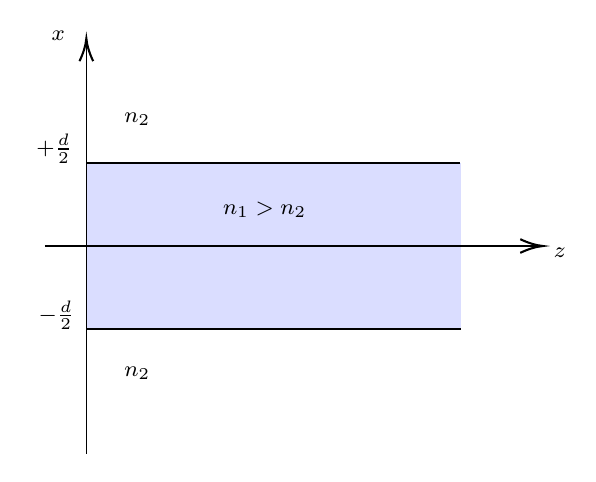
\begin{tikzpicture}[x=0.75pt,y=0.75pt,yscale=-1,xscale=1]
        %uncomment if require: \path (0,310); %set diagram left start at 0, and has height of 310
        
        %Shape: Rectangle [id:dp439999456910388] 
        \draw  [draw opacity=0][fill={rgb, 255:red, 218; green, 221; blue, 255 }  ,fill opacity=1 ] (100,80) -- (280.5,80) -- (280.5,160) -- (100,160) -- cycle ;
        %Shape: Boxed Line [id:dp5082075899729874] 
        \draw    (80,120) -- (318,120) ;
        \draw [shift={(320,120)}, rotate = 180] [color={rgb, 255:red, 0; green, 0; blue, 0 }  ][line width=0.75]    (10.93,-3.29) .. controls (6.95,-1.4) and (3.31,-0.3) .. (0,0) .. controls (3.31,0.3) and (6.95,1.4) .. (10.93,3.29)   ;
        %Shape: Boxed Line [id:dp5101173446407539] 
        \draw    (100,220) -- (100,22) ;
        \draw [shift={(100,20)}, rotate = 450] [color={rgb, 255:red, 0; green, 0; blue, 0 }  ][line width=0.75]    (10.93,-3.29) .. controls (6.95,-1.4) and (3.31,-0.3) .. (0,0) .. controls (3.31,0.3) and (6.95,1.4) .. (10.93,3.29)   ;
        %Shape: Boxed Line [id:dp2709424820833741] 
        \draw    (100.5,160) -- (280.5,160) ;
        %Shape: Boxed Line [id:dp10541842748284669] 
        \draw    (100,80) -- (280,80) ;
        
        
        % Text Node
        \draw (74.67,64.73) node [anchor=north west][inner sep=0.75pt]  [font=\footnotesize]  {$+\frac{d}{2}$};
        % Text Node
        \draw (72,145.07) node [anchor=north west][inner sep=0.75pt]  [font=\footnotesize]  {$\ -\frac{d}{2}$};
        % Text Node
        \draw (164.67,97.73) node [anchor=north west][inner sep=0.75pt]  [font=\footnotesize]  {$n_{1}  >n_{2}$};
        % Text Node
        \draw (117,177.07) node [anchor=north west][inner sep=0.75pt]  [font=\footnotesize]  {$n_{2}$};
        % Text Node
        \draw (117,54.4) node [anchor=north west][inner sep=0.75pt]  [font=\footnotesize]  {$n_{2}$};
        % Text Node
        \draw (324,119.73) node [anchor=north west][inner sep=0.75pt]  [font=\footnotesize]  {$z$};
        % Text Node
        \draw (82,15.07) node [anchor=north west][inner sep=0.75pt]  [font=\footnotesize]  {$x$};
        
        
        \end{tikzpicture}
        
        \end{figure}
          
        Figure \ref{fig_planarwave} shows a planar waveguide consisting of two materials with refractive indices $n_1$ for the core and $n_2$ for the cladding. This waveguide is infinite in the y-direction, has a thickness $d$ (which satisfies that $d >> \lambda$), and fulfills the total internal reflection condition at the boundary \citep{yariv_b}, \citep{OKAMOTO200613}.  Its transverse propagation constant is
        
        
                    \begin{equation}
                        h=\sqrt{k_0^2n_1^2-\beta^2},
                        \label{eq_h}
                    \end{equation}
         where $\beta$ and $h$ are for the core region. For the cladding region, we have the longitudinal propagation constant $\kappa$
        
                     \begin{equation}
                        \kappa=\sqrt{\beta^2-k_0^2n_2^2}.
                        \label{gam}
                    \end{equation}
         
         Here $k_0 = \omega_0/c$ is the wavenumber in vacuum.
        
        
        
        We can include U, W, and V
        
                    \begin{equation}
                        U^2+W^2 = V^2 = k_0^2a^2(n_1^2-n_2^2) \
                        \begin{cases}
                            U = a \times h \\
                            W = a \times \kappa
                        \end{cases} 
                        \label{Normv},
                    \end{equation}
        where V is the so-called waveguide parameter or normalized frequency. 
        The TE mode is then given by 
                 
                    
                    \begin{equation}
                    \textbf{TE mode} \ \ W=
                        \begin{cases}
                            U \tan(U) & \text{even mode}\\
                            -U cotan(U) & \text{odd mode}
                        \end{cases}
                        \label{Temode}
                    \end{equation}
        
        We can solve the eigenvalue problem graphically by plotting W as a function of U [Joly's lecture]. Figure \ref{fig:eigen1} shows this approach where the circle has a radius of V.
        
        
        \begin{figure}[label={fig:eigen1}, caption={Visualization of the graphic solution of the eigenvalue problem. Taken from \cite{herokuapp}}]
          %  \caption*{Source: Some Source}
        	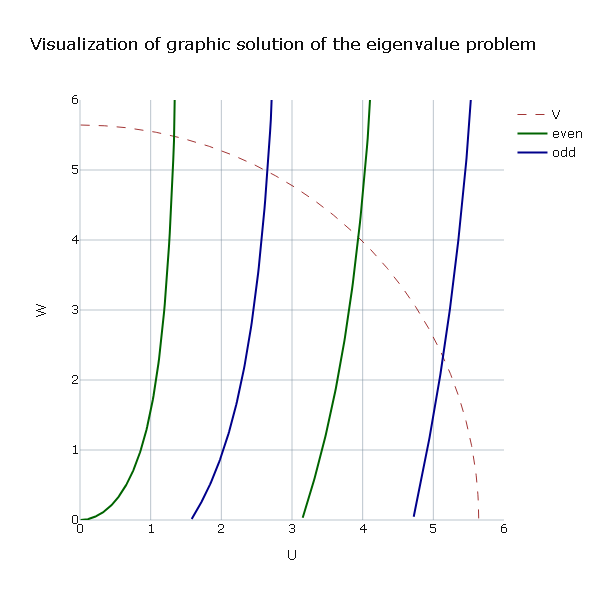
\includegraphics[width=.6\textwidth]{figures/chap2/Eigenvalue.png} 
        \end{figure}
        
        We created a code at the Max-Plank institute \cite{gitmax} to show the students how a change of parameters can affect the plot and, thus, the solutions of the eigenvalue problem. This web tool aims to help the students understanding this problem, and figure \ref{fig:planarp}  shows the interface. The code is written in Python and the Web interface made with Dash/Plotly.  
        
        \begin{figure}[label={fig:planarp}, caption={\href{https://fiber-mode-app.herokuapp.com/apps/dash_plot}{Heroku app} for the planar waveguide.}]
          %  \caption*{Source: Some Source}
        	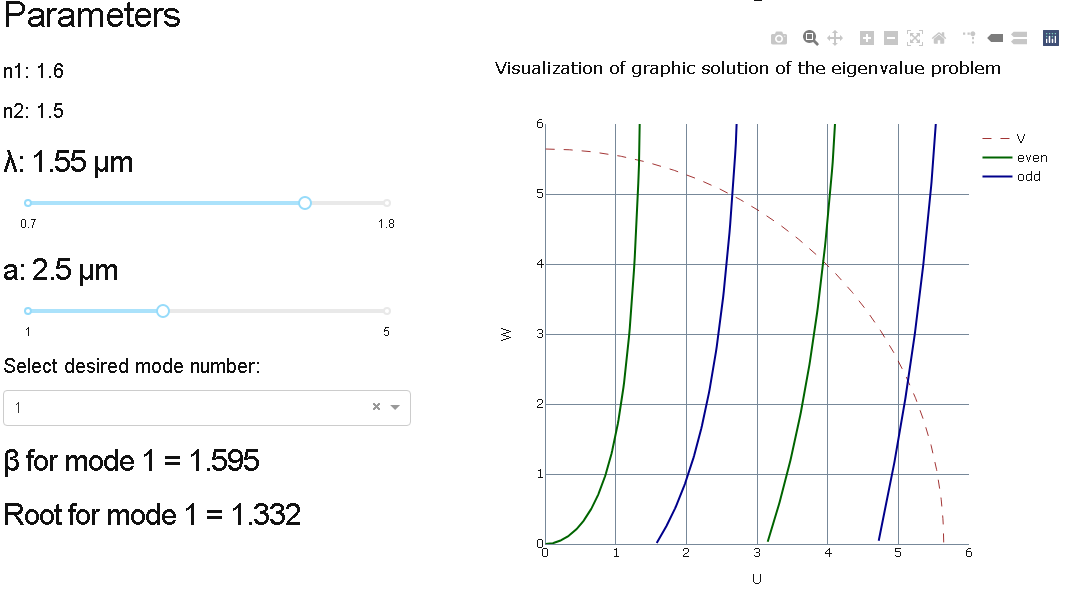
\includegraphics[width=.8\textwidth]{figures/chap2/planarpage.png} 
        \end{figure}
        
        
        Heroku is a web that supports programming languages like Java, Node.js, Python, among others \cite{heorku}. The codes for the planar waveguide and the optical fiber were deployed using its free service.

    \subsection{Optical Fiber}
    
        The code can also solve the problem for the optical fiber, and the students can change some more parameters like cladding and core material, see the Poynting vector or some of the cuts of the field. Figures \ref{fig:fibre1} and \ref{fig:fibre2} show this web. 
        
        
        The refractive index of a material can be approximated by 
        \begin{equation}
            n^2 (\omega) = 1 + \sum_{j=1}^{m} \frac{B_j\omega^2_j}{\omega^2_j - \omega^2} 
            \label{eq_ene}
        \end{equation}
        called the Sellmeier equation. Here $\omega_j$ is the resonance frequency and $B_j$ the strength of it \citep{AgrawalBook}. This allowed to add the different materials to de code an can be changed by selecting the material in the dropwdowns for the core and the cladding of the fiber.
        
        
        \begin{figure}[label={fig:fibre1}, caption={\href{https://fiber-mode-app.herokuapp.com/apps/results}{Heroku app} for the optical fiber (1).}]
          %  \caption*{Source: Some Source}
        	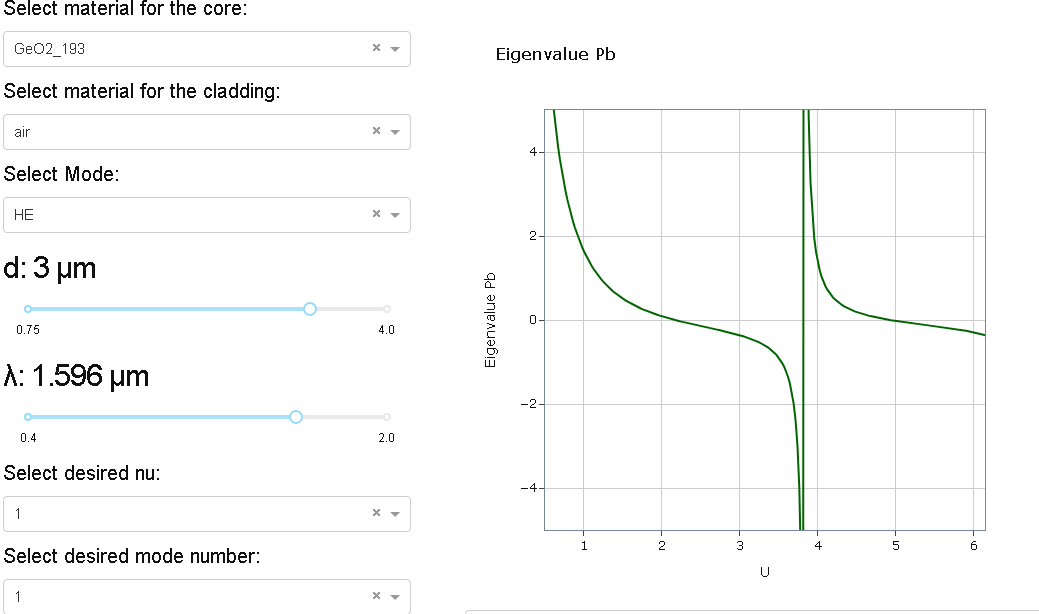
\includegraphics[width=.8\textwidth]{figures/chap2/fibre1.PNG} 
        \end{figure}
        
        \begin{figure}[label={fig:fibre2}, caption={\href{https://fiber-mode-app.herokuapp.com/apps/results}{Heroku app} for the optical fiber (2).}]
          %  \caption*{Source: Some Source}
        	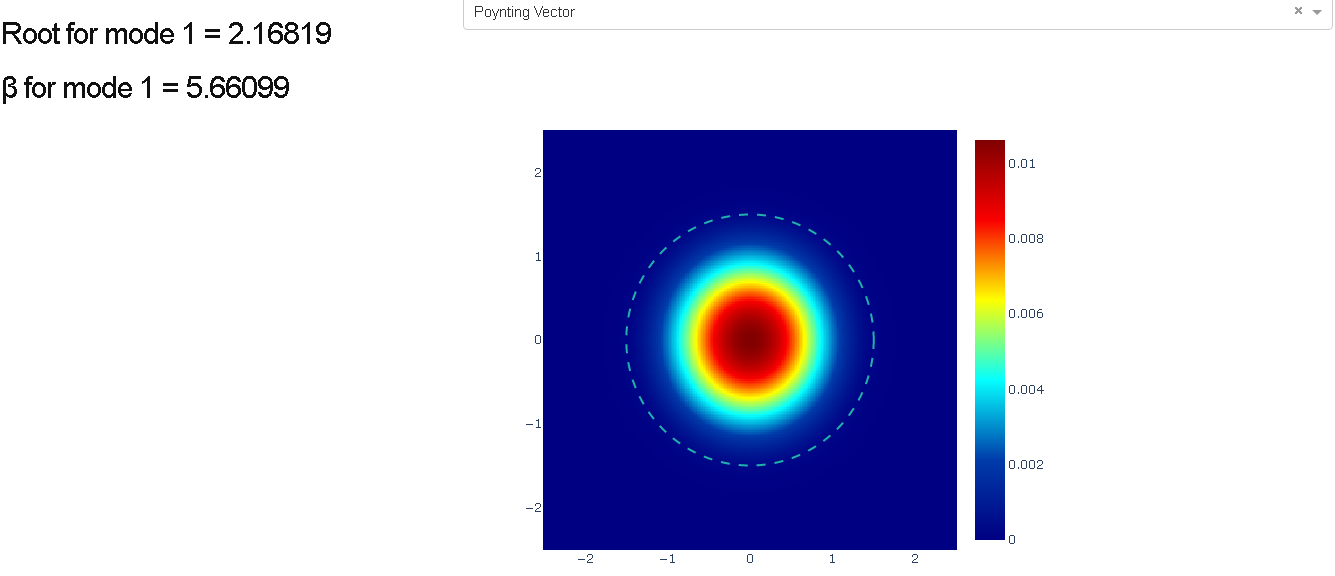
\includegraphics[width=.8\textwidth]{figures/chap2/fibre2.PNG} 
        \end{figure}
    

   


\section{Pulse propagation in fibers}

Loss and dispersion originated by interactions of the electromagnetic field with the atoms of the medium, and frequency dependence of the refractive index affect the propagation of an electromagnetic wave through this medium \citep{dudley_taylor_2010}. Shape and spectrum of short pulses with widths between approx. 10ns and 10fs propagating in a fiber are affected by nonlinear and dispersive effects \citep{AgrawalBook}.  

    \subsection{Pulse evolution inside a single-mode fiber:}
        The slowly varying amplitude \emph{A(z,t)} can be described by the equation:
        \begin{equation}\label{eq_a}
        \begin{split}
            \frac{\partial A}{\partial z}&= \overbrace{-\frac{\alpha}{2} - \beta_1\frac{\partial A}{\partial t} - \frac{i \beta_2}{2} \frac{\partial^2 A}{\partial t^2} +\frac{\beta_3}{6} \frac{\partial^3 A}{\partial t^3}}^{\mathbf{linear \ effects}}\\  
            & +\underbrace{i \gamma \left( 1 + \frac{i}{\omega_0} \frac{\partial}{\partial t} \right) \left( A(z,t) \int_{-\infty}^{\infty} R(t') \left|A(z, t-t') \right|^2 \ dt'  \right)}_{\mathbf{nonlinear \ effects}}
        \end{split}
        \end{equation}
    %[A] = sqrt(W)
    where: 
    \begin{itemize}
        \item \textbf{t} is the time variable [s]
        \item \textbf{z} is the space variable [m]
        \item $\mathbf{\alpha}$ is the attenuation coefficient [1/m]
        \item $\mathbf{\beta_n}$ are propagation constant coefficients $[s^n/m]$
        \item $\mathbf{\gamma}$ is the nonlinear parameter [1/Wm]
        
            \begin{equation}
                \gamma = \frac{n_2 \omega_0}{c A_{eff}},
                \label{eq_gamma}
            \end{equation}
        with $\mathbf{n_2} \quad [m^2/W]$ which is the nonlinear refractive index, and $A_{eff} \quad [m^2]$ that  is the  effective core area.
        %or  n2 is the nonlinear-index coefficient. 
        \item \textbf{R(t)} [1/s] is the response function that includes electronic and vibrational contributions and is approximated by 
        
        \begin{equation}\label{eq_rt}
            R(t) = (1- f_R)\delta(t) + f_R h_R(t),
        \end{equation}
        where $f_R$ and $h_R(t)$ are the fractional contribution of the delayed Raman response and the Raman response function, respectively. Conforming to \cite{dudley_taylor_2010}, 
        \begin{equation}\label{eq_hr}
            h_R(t) = \frac{\tau^2_1+\tau^2_2}{\tau_1\tau^2_2} exp(-t/\tau_2)sin(t/\tau_1)\Theta(t),
        \end{equation}
        here $\delta(t)$ and $\Theta(t)$ are the Delta Dirac and the Heaviside step functions, respectively; $f_R = 0.18$,  $\tau_1 =12.2 fs$, and $\tau_2 = 32 fs$.
         
         
        \item $\omega_0$  is the center angular frequency
    
    \end{itemize}
   
    One can asume that the evolution of the envelope pulse is slow, and remembering that the group velocity is defined by 
    
    \begin{equation}\label{eq_vg}
        v_g \equiv \frac{1}{\beta_1}, 
    \end{equation}
    and the pulse can be moved at the group velocity using the reference frame 
    \begin{equation}\label{eq_t}
        T = t - \frac{z}{v_g}. 
    \end{equation}
    
    Thus, equation \eqref{eq_a} can be defined as 
    
    \begin{equation}\label{eq_b}
        \frac{\partial A}{\partial z}=-\frac{\alpha}{2} - \frac{i \beta_2}{2}A \frac{\partial^2 A}{\partial T^2} +\frac{\beta_3}{6} \frac{\partial^3 A}{\partial T^3} +i \gamma   \left(A\left|A\right|^2+ \frac{i}{\omega_0} \frac{\partial}{\partial T} (A\left|A \right|^2)- A \ T_R \frac{\partial \left|A \right|^2}{\partial T} \right),
        \end{equation}
    where the first moment of the nonlinear (Raman) response is
    \begin{equation}\label{eq_TR}
        T_R = f_R\int_{0}^{\infty} t \ h_R(t) \ dt.
    \end{equation}

        
    \subsection{Nonlinear Schrödinger Equation}
        According to \citep{AgrawalBook}, the equation  \eqref{eq_b} for the slowly varying envelope can be simplified for pulses of width $T_0 > 5 ps$ to
        \begin{equation}
                \frac{\partial A}{\partial z} = -\frac{\alpha}{2}A-j \frac{\beta_2}{2}\frac{\partial^2A}{\partial T^2}+j\gamma|A|^2 A,
                \label{eq_nlse}
            \end{equation}
            \ \\
       It is noteworthy that the contribution of the third-dispersion term should be considered if $\beta_2 \approx 0$ (zero-dispersion region). Equation \eqref{eq_nlse} is known as the nonlinear \gls{NLSE}. %Schrödinger equation (NLSE).

           Following the convention used in \cite{AgrawalBook}, \cite{dudley_taylor_2010} , the continuous inverse Fourier transform of the slowly varying function of z is
        
        \begin{equation}\label{eq_acft}
            A(z,t) = \frac{1}{2\pi} \int_{-\infty}^{\infty} %\tilde{A}(z,\omega-\omega_0)\exp{[-i(\omega-
            \tilde{A}(z,\omega)exp(-i\omega t) \ d\omega \ .
        \end{equation}
        
        
        The \Gls{FFT} is an algorithm capable of calculating the \Gls{DFT} faster \citep{Lynch2018}. The definition of \href{https://numpy.org/doc/stable/index.html}{Numpy} of the inverse \Gls{DFT} as \cite{dft} says is 
        \begin{equation}\label{eq_dft}
            a_n = \frac{1}{n}\sum_{k=0}^{n-1} A_k \ exp\left\{ 2\pi i \frac{mk}{n} \right\} \qquad m = 0,...,n-1,
        \end{equation}

        then, it follows
        \begin{equation} \label{eq_deffft}
                A(z,T) = FFT \left[ \tilde{A}(z,\omega) \right].
            \end{equation}
            
            
    \subsection{Dispersion}
        The frequency dependency of the refractive index can lead to different speeds of propagation from different wavelengths of pulses in a fiber, which causes a broadening of the pulse in the time domain. This effect can limit the transmission of information and generate effects like inter symbol interference.  So, one can call chromatic dispersion the delay between several spectral components of a traveling pulse, i.e., there are different group velocities for the diverse components propagating in the fiber  \citep{Udayakumar2013ChromaticDC}. This delay depends on the waveguide (e.g., core radius) and material (e.g., the difference between core and cladding indices) contributions \citep{dudley_taylor_2010}. 
        
        The Taylor series expansion of the propagation constant 
        \begin{equation}
             \beta(\omega) = n (\omega)\frac{\omega}{c} = \beta_0 + \beta_1(\omega-\omega_0) \frac{1}{2}\beta_2(\omega-\omega_0)^2+...\, 
             \label{eq_betas}
        \end{equation}
        with 
        \begin{equation}
            \beta_m = \frac{d^m\beta}{d\omega^2}_{\omega = \omega_0} \qquad (m = 0,1,2,...),
            \label{eq_dbeta}
        \end{equation}
        
        
        defines the \gls{GVD} parameter $\beta_2$  and higher-order dispersion terms.  $\beta_2$ is also related to the dispersion parameter D by
        \begin{equation}
            D = \frac{d\beta_1}{d\lambda} = - \frac{2\pi c}{\lambda^2}\beta_2 \quad [\frac{ps}{nm \ km}] \ .
            \label{eq_Ds}
        \end{equation}
        
        Depending on the value of the \Gls{GVD} parameter, either shows the fiber a normal dispersion ($\beta_2 > 0$ , $D<0$), or it is in the anomalous dispersion regime ($\beta_2 < 0$ , $D>0$).
        
        Linear solitons can reduce this effect, even though there are several methods to compensate chromatic dispersion, as \cite{AgrawalBook}, \cite{dudley_taylor_2010},  and \citep{Udayakumar2013ChromaticDC} explain.
        \gls{DCF}, Fiber Bragg Grating (FBG), and Optical Phase Conjugator (OPC) are some of the methods used.
        
       

    \subsection{Nonlinear Effects}

        Nonlinearities can be effects such as third-harmonic generation, four-wave mixing (FWM). The Kerr nonlinearity $n = n(P_{opt})$
        can lead to a time-dependent phase delay of the pulse itself, known as self-phase modulation, to a co-propagating pulse, known as cross-phase modulation (XPM), or the formation of a fourth component through up to three light waves with different frequencies (FMW ) \cite{rein}. The refractive index is written as
        
        
        \begin{equation}
            \tilde{n} (\omega, \left| E \right|^2) = \overbrace{n(\omega)}^{linear \ part \ Eq. \ \eqref{eq_ene}} + \underbrace{ n_2 \left| E \right|^2}_{nonlinear part},
        \end{equation} 
       
       where $n_2 = \frac{3}{8n}Re\left\{ \chi^{(3)}_{\chi \chi \chi}\right\}$ and $\chi^{(3)}$ is the third-order susceptibility.
   
   \subsubsection{Stimulated Inelastic Scattering}
        A further aspect of the nonlinear effects is the stimulated inelastic scattering. These effects are the stimulated Raman and Brillouin scattering (SRS and SBS, respectively). Vibrations of the molecular bonds of the medium interact with the injected pulse, which can lead to an amplification of the "Stokes wave" through a scattering power transfer by the molecular vibrations \cite{rein}. A main difference is that SRS and SBS involve then optical and acoustic phonons, respectively \cite{AgrawalBook}.
        
    \subsection{Optical Solitons}
    
    
    Solving the NLSE can involve the appearance of solitons when nonlinear effects (in general arising from the Kerr-effect) act together with the GVD. The invariance of amplitude and velocity is a relevant characteristic of the solitons. However, their phase and position are not invariant \cite{Kodama1994}. 
    
    The existence of dark and bright solitons depends on whether the GVD is in the normal (or positive) regime for the first case or in the anomalous region for the bright type \cite{KIVSHAR199881}, \cite{agr_pap}.  When the amplitude envelope of the pulse has a localized dip of the pulse (whose drop reaches zero intensity), the solution of the NLSE is called a "dark" soliton. These dark-soliton pulses can fade because of the Raman self-scattering, even though the background fluctuations and loss are stronger in bright than in dark solitons \cite{kivshar}. 
    
    Dark solitons can be converted into bright solitons by employing a micro-ring resonator, which, in turn, is particularly similar to a Fabry Perot resonator \cite{yupapin}. This conversion may have applications for network security (due to the difficult detection of the dark pulse propagating through the port) \cite{darkks}. Using a resonator system with soliton pulses leads to a broadening of the spectrum of light. Its applications can be security imaging, medical tools, multi-color holography, and transparent holography \cite{yupapin}.
%%%%%%%%%%%%%%%%%%%%%%%%%%%%%%%%%%%%%%%%%%%%%%%%%%%%%%%%%%%%55

\section{Solution of the NLSE}

    It is common to solve the nonlinear differential equations \eqref{eq_b} and \eqref{eq_nlse} by a numerical method instead of analytical methods like \citep{Mihalache_1993}.  


    \subsection{Step-Doubling Technique}
         \citep{dudley_taylor_2010} uses an adaptative algorithm to propagate the solution of the NLSE having two steps of calculation and a longer one equivalent starting at the same point. Therefore, they estimate the error through the differences between computations to converge more quickly. In \citep{gitdud}  is presented a Matlab-based code using this step-doubling technique. 
         
    \subsection{Split-Step Fourier Method}

        In this thesis, the split-step Fourier method (SSFM) was the numerical method selected to solve the NLSE. \citep{AgrawalBook}, \citep{sinkin}, \citep{robust},  and \citep{HohageSchmidt2002} show different approaches and points of view of this method.  \citep{robust} gives a robust SSFM,  \citep{sinkin} explains how to select optimized step sizes depending on the accuracy or effect desired to inspect with the SSFM, and  \citep{HohageSchmidt2002} offers a comparison between the different kinds of SSFM. Furthermore, Suárez, P. \citep{suarez} gives a MATLAB implementation of the SSFM with a learning and teaching perspective. 
        
        Following \citep{AgrawalBook}, equations \eqref{eq_b} and \eqref{eq_nlse} can be represented by using
    
        \begin{equation}\label{eq_dpn}
            \frac{\partial A}{\partial z} = \left( \hat{\mathcal{D}} + \hat{\mathcal{N}} \right) A, 
        \end{equation}
        
        with $\hat{\mathcal{D}}$ known as the differential operator, and $\hat{\mathcal{N}}$ as the nonlinear operator: 
        
        \begin{equation} \label{eq_dhat}
            \hat{\mathcal{D}} = -\frac{\alpha}{2} - \frac{i \beta_2}{2} \frac{\partial^2 }{\partial T^2} +\frac{\beta_3}{6} \frac{\partial^3 }{\partial T^3},
        \end{equation}
        and
        \begin{equation} \label{eq_nhat}
             \hat{\mathcal{N}} = i \gamma   \left(\left|A\right|^2+ \frac{i}{\omega_0} \frac{\partial}{\partial T} (\left| A\right|^2)-  \ T_R \frac{\partial \left|A \right|^2}{\partial T} \right).
        \end{equation}
        
        One can approximate the solution of the NLSE by splitting the fiber into pieces of a length of size $h$ and assuming that the dispersive and nonlinear effects operate separately. I.e., the nonlinearities act alone ($\hat{\mathcal{D}} = 0$) and, during the second step, their roles change by setting $\hat{\mathcal{N}} = 0$.

        The pulse propagates from $z$ to $z+h$ employing the equation 
        
        \begin{equation}\label{eq_azh}
            A(z+h, T) \approx e^{h\hat{\mathcal{D}}} e^{h\hat{\mathcal{N}}} A(z,T) \ ,
        \end{equation}
        
        or the symmetric SSFM \citep{sinkin}
        \begin{equation}\label{eq_azh2}
            A(z+h, T) \approx e^{\frac{h}{2}\hat{\mathcal{D}}} e^{\frac{h}{2}\hat{\mathcal{N}}} e^{\frac{h}{2}\hat{\mathcal{D}}} A(z,T) \ .
        \end{equation} According to \citep{Balac2013OverviewOA}, this method requires an adequate adaptive step-size control scheme because it presents a strong dependency on the grid points used. Figure \ref{fig_ssfmd} depicts the Symmetric SSFM.
        
        
        
        
         \begin{figure}[label={fig_ssfmd}, caption={Sketch of a Symmetric SSFM. Adapted from \citep{Balac2013OverviewOA}.}]
                  %  \caption*{Source: Some Source}
                \centering  
%\tikzset{every picture/.style={line width=0.75pt}} %set default line width to 0.75pt        
        
        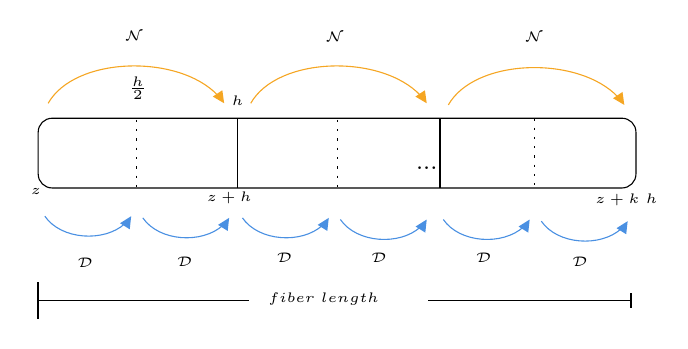
\begin{tikzpicture}[x=1.2pt,y=1.2pt,yscale=-1,xscale=1]
        %uncomment if require: \path (0,300); %set diagram left start at 0, and has height of 300
            
            %Rounded Rect [id:dp3852932235223505] 
            \draw   (100,115.2) .. controls (100,112.88) and (101.88,111) .. (104.2,111) -- (275.8,111) .. controls (278.12,111) and (280,112.88) .. (280,115.2) -- (280,127.8) .. controls (280,130.12) and (278.12,132) .. (275.8,132) -- (104.2,132) .. controls (101.88,132) and (100,130.12) .. (100,127.8) -- cycle ;
            %Straight Lines [id:da004144927883721339] 
            \draw    (160,111) -- (160,132) ;
            %Straight Lines [id:da3654232899891592] 
            \draw    (221,111) -- (221,132) ;
            %Straight Lines [id:da45475006001951823] 
            \draw    (100,166) -- (163.5,166) ;
            \draw [shift={(100,166)}, rotate = 180] [color={rgb, 255:red, 0; green, 0; blue, 0 }  ][line width=0.75]    (0,5.59) -- (0,-5.59)   ;
            %Straight Lines [id:da9346841303105087] 
            \draw    (217.5,166) -- (278.5,166) ;
            \draw [shift={(278.5,166)}, rotate = 180] [color={rgb, 255:red, 0; green, 0; blue, 0 }  ][line width=0.75]    (0,2.24) -- (0,-2.24)   ;
            %Curve Lines [id:da5361939697011324] 
            \draw [color={rgb, 255:red, 245; green, 166; blue, 35 }  ,draw opacity=1 ]   (103,106.5) .. controls (111.03,92.32) and (142.28,91.55) .. (154.14,104.16) ;
            \draw [shift={(156,106.5)}, rotate = 236.31] [fill={rgb, 255:red, 245; green, 166; blue, 35 }  ,fill opacity=1 ][line width=0.08]  [draw opacity=0] (3.57,-1.72) -- (0,0) -- (3.57,1.72) -- cycle    ;
            %Straight Lines [id:da41945250802592127] 
            \draw  [dash pattern={on 0.84pt off 2.51pt}]  (129.5,111.5) -- (129.5,132.5) ;
            %Straight Lines [id:da9865879096776455] 
            \draw  [dash pattern={on 0.84pt off 2.51pt}]  (190,111.5) -- (190,132.5) ;
            %Straight Lines [id:da5596453819308491] 
            \draw  [dash pattern={on 0.84pt off 2.51pt}]  (249.5,111) -- (249.5,132) ;
            %Curve Lines [id:da018780585468089805] 
            \draw [color={rgb, 255:red, 245; green, 166; blue, 35 }  ,draw opacity=1 ]   (164,106.5) .. controls (172.03,92.32) and (203.28,91.55) .. (215.14,104.16) ;
            \draw [shift={(217,106.5)}, rotate = 236.31] [fill={rgb, 255:red, 245; green, 166; blue, 35 }  ,fill opacity=1 ][line width=0.08]  [draw opacity=0] (3.57,-1.72) -- (0,0) -- (3.57,1.72) -- cycle    ;
            %Curve Lines [id:da8889794263264403] 
            \draw [color={rgb, 255:red, 245; green, 166; blue, 35 }  ,draw opacity=1 ]   (223.5,107) .. controls (231.53,92.82) and (262.78,92.05) .. (274.64,104.66) ;
            \draw [shift={(276.5,107)}, rotate = 236.31] [fill={rgb, 255:red, 245; green, 166; blue, 35 }  ,fill opacity=1 ][line width=0.08]  [draw opacity=0] (3.57,-1.72) -- (0,0) -- (3.57,1.72) -- cycle    ;
            %Curve Lines [id:da109759730738193] 
            \draw [color={rgb, 255:red, 74; green, 144; blue, 226 }  ,draw opacity=1 ]   (102,140.5) .. controls (106.92,147.66) and (119.86,148.41) .. (126.1,142.76) ;
            \draw [shift={(128,140.5)}, rotate = 482.01] [fill={rgb, 255:red, 74; green, 144; blue, 226 }  ,fill opacity=1 ][line width=0.08]  [draw opacity=0] (3.57,-1.72) -- (0,0) -- (3.57,1.72) -- cycle    ;
            %Curve Lines [id:da5801862642922446] 
            \draw [color={rgb, 255:red, 74; green, 144; blue, 226 }  ,draw opacity=1 ]   (131.5,141) .. controls (136.42,148.16) and (149.36,148.91) .. (155.6,143.26) ;
            \draw [shift={(157.5,141)}, rotate = 482.01] [fill={rgb, 255:red, 74; green, 144; blue, 226 }  ,fill opacity=1 ][line width=0.08]  [draw opacity=0] (3.57,-1.72) -- (0,0) -- (3.57,1.72) -- cycle    ;
            %Curve Lines [id:da32600514781734646] 
            \draw [color={rgb, 255:red, 74; green, 144; blue, 226 }  ,draw opacity=1 ]   (161.5,141) .. controls (166.42,148.16) and (179.36,148.91) .. (185.6,143.26) ;
            \draw [shift={(187.5,141)}, rotate = 482.01] [fill={rgb, 255:red, 74; green, 144; blue, 226 }  ,fill opacity=1 ][line width=0.08]  [draw opacity=0] (3.57,-1.72) -- (0,0) -- (3.57,1.72) -- cycle    ;
            %Curve Lines [id:da574569055792788] 
            \draw [color={rgb, 255:red, 74; green, 144; blue, 226 }  ,draw opacity=1 ]   (191,141.5) .. controls (195.92,148.66) and (208.86,149.41) .. (215.1,143.76) ;
            \draw [shift={(217,141.5)}, rotate = 482.01] [fill={rgb, 255:red, 74; green, 144; blue, 226 }  ,fill opacity=1 ][line width=0.08]  [draw opacity=0] (3.57,-1.72) -- (0,0) -- (3.57,1.72) -- cycle    ;
            %Curve Lines [id:da16955896501211276] 
            \draw [color={rgb, 255:red, 74; green, 144; blue, 226 }  ,draw opacity=1 ]   (222,141.5) .. controls (226.92,148.66) and (239.86,149.41) .. (246.1,143.76) ;
            \draw [shift={(248,141.5)}, rotate = 482.01] [fill={rgb, 255:red, 74; green, 144; blue, 226 }  ,fill opacity=1 ][line width=0.08]  [draw opacity=0] (3.57,-1.72) -- (0,0) -- (3.57,1.72) -- cycle    ;
            %Curve Lines [id:da7109799228168221] 
            \draw [color={rgb, 255:red, 74; green, 144; blue, 226 }  ,draw opacity=1 ]   (251.5,142) .. controls (256.42,149.16) and (269.36,149.91) .. (275.6,144.26) ;
            \draw [shift={(277.5,142)}, rotate = 482.01] [fill={rgb, 255:red, 74; green, 144; blue, 226 }  ,fill opacity=1 ][line width=0.08]  [draw opacity=0] (3.57,-1.72) -- (0,0) -- (3.57,1.72) -- cycle    ;
            
            % Text Node
            \draw (111,152.4) node [anchor=north west][inner sep=0.75pt]  [font=\tiny]  {$\mathcal{D}$};
            % Text Node
            \draw (141,151.9) node [anchor=north west][inner sep=0.75pt]  [font=\tiny]  {$\mathcal{D}$};
            % Text Node
            \draw (171,150.9) node [anchor=north west][inner sep=0.75pt]  [font=\tiny]  {$\mathcal{D}$};
            % Text Node
            \draw (199.5,150.9) node [anchor=north west][inner sep=0.75pt]  [font=\tiny]  {$\mathcal{D}$};
            % Text Node
            \draw (231,150.9) node [anchor=north west][inner sep=0.75pt]  [font=\tiny]  {$\mathcal{D}$};
            % Text Node
            \draw (260,151.9) node [anchor=north west][inner sep=0.75pt]  [font=\tiny]  {$\mathcal{D}$};
            % Text Node
            \draw (125.5,83.9) node [anchor=north west][inner sep=0.75pt]  [font=\tiny]  {$\mathcal{N}$};
            % Text Node
            \draw (186,84.4) node [anchor=north west][inner sep=0.75pt]  [font=\tiny]  {$\mathcal{N}$};
            % Text Node
            \draw (246,84.4) node [anchor=north west][inner sep=0.75pt]  [font=\tiny]  {$\mathcal{N}$};
            % Text Node
            \draw (97,131.4) node [anchor=north west][inner sep=0.75pt]  [font=\tiny]  {$z$};
            % Text Node
            \draw (150,132.4) node [anchor=north west][inner sep=0.75pt]  [font=\tiny]  {$z+h$};
            % Text Node
            \draw (267,132.9) node [anchor=north west][inner sep=0.75pt]  [font=\tiny]  {$z+k\ h$};
            % Text Node
            \draw (213,124.9) node [anchor=north west][inner sep=0.75pt]  [font=\small]  {$...$};
            % Text Node
            \draw (168.5,162.9) node [anchor=north west][inner sep=0.75pt]  [font=\tiny]  {$fiber\ length$};
            % Text Node
            \draw (126.5,97.9) node [anchor=north west][inner sep=0.75pt]  [font=\tiny]  {$\frac{h}{2}$};
            % Text Node
            \draw (157.5,103.4) node [anchor=north west][inner sep=0.75pt]  [font=\tiny]  {$h$};
            
                
            \end{tikzpicture}
        \end{figure}
        
%Write eq for propagation and explain LD vs LNL Bereiche ->  GVD only -> U(0,T) Gauss- und Sech-Pulse -> wie wird das Programm durchgeführt? Ergebnisse mithilfe Matplotlibs, und Darstelung in einer Web-App 
		\chapter{Creation of the Web-tool}



 \section{Modeling the short  pulse propagation}
    In order to have an easier understanding of the physical processes involved in the propagation of short pulses in a medium, it will be first necessary to focus on the dispersion that affects this medium. The purpose of this section is to consider the fiber as a linear optical medium while studying the pulse-propagation problem. Thus, it is possible to inspect the effect of GVD under certain circumstances where it dominates over the nonlinearities \citep{ AgrawalBook}. A further objective of this thesis is to implement a code capable of illustrating the Dispersion-induced broadening of optical pulses for both Gaussian and Hyperbolic-Secant (Sech) shapes.


    In this work, the normalized amplitude \emph{U} will be used and is obtained from  
  
            \begin{equation}\label{eq_A0}
                A(z,\tau ) = \sqrt{P_0}e^{\frac{-\alpha z}{2}} U(z,\tau) \ ,
            \end{equation}
            with
            \begin{equation}
                \tau =  \frac{T}{T_0} = \frac{t-z/v_g}{T_0} \ ,
            \end{equation}
        
        which is the time scale scaled to the input pulse width $T_0$.
        
        
        It is important to define relative lengths in order to understand the effect of the dispersion and/or nonlinearities on a pulse propagation
            \ \\
            \ \\
            \begin{equation}
                L_D = \frac{T^2_0}{|\beta_2|} \qquad and \qquad L_{NL} = \frac{1}{\gamma P_0} \ ,
            \end{equation}
        
        where $L_D$ is known as the dispersion length and $L_{NL}$ as the nonlinear length. Hence, the propagation of a pulse can present four different regimes depending on the length L of the fiber. This differentiation allows us to inspect the distinct phenomenon individually. Therefore, the students can comprehend how the pulse is affected by either the dispersion or the nonlinearities. The four regimes are 
        \begin{equation}
            \begin{aligned}\label{eq_lregimes}
               \mathbf{1} \quad L \ll L_D \quad & \quad L \ll  L_{NL} \ , \\
              \mathbf{2} \ \quad L \approx L_D \quad & \quad L \ll  L_{NL} \ , \\
               \mathbf{3} \quad L \ll L_D \quad & \quad L \approx  L_{NL} \ , \\
               \mathbf{4} \quad L \gg L_D \quad & \quad L \gg  L_{NL} \ . \\
            \end{aligned}
        \end{equation} 
        
        For the first case, both effects are negligible. In the second and third cases, the dispersion and nonlinearities act alone, respectively; and finally, both effects play an important role in the fourth case.
        
        \subsection{Modeling the effect of GVD}\label{subsect:gvd}
   
    
        
        Supposing a fiber length L such as $L \sim L_D$, $L << L_{NL}$, and setting $\gamma = 0$:  the equation \eqref{eq_nlse} becomes 
        
         \begin{equation}\label{eq_ugvd}
            \frac{\partial U}{\partial z} = -j\frac{\beta_2}{2}\frac{\partial^2U}{\partial T^2}.
        \end{equation}

        It is now necessary to define the incident field for the gaussian-like and the hyperbolic-Secant-like Pulses as 
            
        \begin{equation}\label{eq_u0t}
            U(0,T) = 
            \begin{cases}
                exp \left\{ -\frac{1+iC}{2} \left(\frac{T}{2T^2_0} \right)^{2m} \right\} \qquad \text{for Gaussian-shaped pulses}  \\
                \ \\
                sech\left( \frac{T}{T_0}\right) exp \left\{ -\frac{iCT^2}{2T^2_0} \right\} \qquad \text{for Hyperbolic-Secant pulses}.  \\
            \end{cases}
        \end{equation}
        
         Here are considered the initial chirp C for both types of pulses and the generalization for a supper-gaussian pulse, where m = 1 represents a chirped Gaussian pulse.
        
        
        Recalling the Fourier-transform method \eqref{eq_acft}, the equation \eqref{eq_ugvd} turns out to be the ordinary differential equation
        
        \begin{equation}\label{eq_ugvdw}
            i\frac{\partial\tilde{U}}{\partial z} = \frac{1}{2} \beta_2 \omega^2 \tilde{U} \ .
        \end{equation}
        
        Eventually, one can write the solution of the equation \eqref{eq_ugvdw} as
        
        \begin{equation}\label{eq_gvdufft}
            U(z,T) = FFT \left[ \tilde{U}(0,\omega) \ exp\{j\frac{\beta_2}{2}\omega^2z\} \right], 
        \end{equation}
        
        with
        
        \begin{equation}\label{eq_uw0gvd}
            \tilde{U}(0,\omega)  = FFT^{-1} \left[ U(0,T)\right] \ , 
        \end{equation}
        
        
        and its implementation in Python is straightforward regardless of the shape of the pulse.
        
        
        Agrawal et al. \citep{AgrawalBook} also propose a way to find the amplitude of a gaussian-shaped pulse at the point z by using 
        
        \begin{equation}\label{eq_ugvdg}
            U(z,T) = \frac{T_0}{(T^2_0 - i \beta z)^{1/2}} exp \left( -\frac{T^2}{2(T^2_0 - i \beta z)} \right) \ .
        \end{equation}
        
        This formula has fewer computational steps and was also added to the code to compare the results.  It is worth mentioning that the equation \eqref{eq_ugvdg} is only valid for unchirped  Gaussian pulses.
             
        Having these equations and using \href{https://numpy.org/}{Numpy}, was written a code to plot the pulse evolution. This code allows the user to change values like $\beta_2$ to see the dispersion-induced broadening. 
        
        \begin{figure}[label={fig:gvdmtp}, caption={Effect of GVD in a Gaussian pulse following Eq. \eqref{eq_ugvdg}.}]
        \centering
        \begin{tabular}[c]{cc}
        \centering
        \begin{subfigure}[b]{.53\textwidth}
		    \centering	
            \includegraphics[width=1\textwidth]{figures/chap3/gvdonlygaus.eps}
            \caption{Using Matplotlib and function \emph{Gaussian\_pulse\_GVD()} of the code.}\label{fig:gvdmtp1}
        \end{subfigure}
        \hfill
        \begin{subfigure}[b]{.53\textwidth}
		    \centering	
            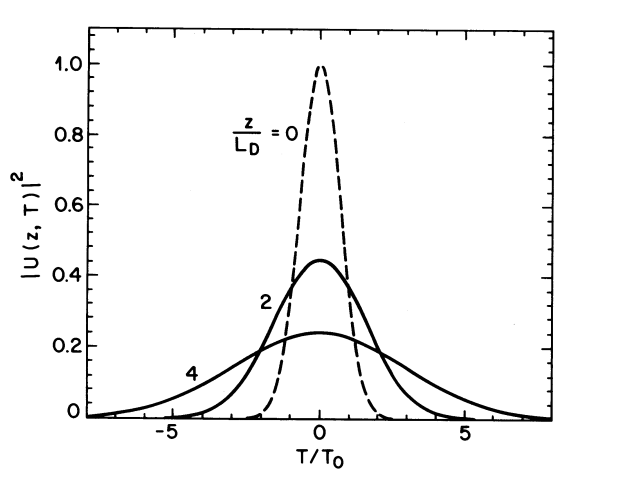
\includegraphics[width=1\textwidth]{figures/chap3/gvdgausagr.png}
            \caption{Plot given in \citep{AgrawalBook} p. 68.}\label{fig:gvdmtp2}
        \end{subfigure}
        \end{tabular}
        \end{figure}
        
        
        \begin{figure}[label={fig:gvdmtps}, caption={Effect of GVD in a Gaussian (Fig. \subref{fig:gvdmtp3}) and in a Sech (Fig. \subref{fig:gvdmtp4}) pulse following Eq. \eqref{eq_gvdufft}, using Matplotlib and function \emph{incident\_field()} of the code.}]
        \centering
        \begin{tabular}[c]{cc}
        \centering
        \begin{subfigure}[b]{.53\textwidth}
		    \centering	
            \includegraphics[width=1\textwidth]{figures/chap3/gvdgaus.eps}
            \caption{Gaussian Pulse.}
            \label{fig:gvdmtp3}
        \end{subfigure}
        \hfill
        \begin{subfigure}[b]{.53\textwidth}
		    \centering	
            \includegraphics[width=1\textwidth]{figures/chap3/gvdsech.eps}
            \caption{Sech Pulse.}
            \label{fig:gvdmtp4}
        \end{subfigure}
        \end{tabular}
        \end{figure}
        
        \subsection{Modeling the effect of SPM}
        The next aspect to understand is the spectral broadening of a pulse because of nonlinear effects. In this case, the phenomenon of SPM influences under a propagation regime such as $ L_D \gg L \sim L_{NL} $, where $\beta_2=0$. The equation \eqref{eq_nlse} becomes: 
            \begin{equation}
                \frac{\partial U}{\partial z} = j\frac{e^{-\alpha z}}{L_{NL}}|U|^2 U \ ,
            \end{equation}
            %seite 98
            which phase shift can be defined as 
            \begin{equation} \label{eq_phi}
                \phi_{NL}(L,T) = |U(0,T)|^2 (L_{eff}/L_{NL})
            \end{equation}
            with 
            \begin{equation} \label{eq_leff}
                L_{eff} = \frac{1-e^{-\alpha L}}{\alpha} \ .
            \end{equation}
            
            If  $\alpha = 0$, then $L_{eff} = L$.
            
            That allow us to introduce the SPM-induced chirp as
            
            \begin{equation} \label{eq_spmchirp}
                \delta \omega(T) = -\frac{\partial \phi_{NL}}{\partial T} = -\left( \frac{L_{eff}}{L_{NL}} \right) \frac{\partial }{T} |U(0,T)|^2 \ ,
            \end{equation}
        
        
         and generalized for a super-Gaussian pulse:
            \begin{equation} \label{eq_spmchirpsg}
                \delta \omega(T) = \frac{2m L_{eff}}{T_0 L_{NL}}\left( \frac{T}{T_0}\right)^{2m-1}  exp\left\{ -\left( \frac{T}{T_0}\right)^{2m}   \right\}
            \end{equation}
        
        The code in Appendix \ref{sec:initvariables} uses the equations \eqref{eq_spmchirp} and \eqref{eq_spmchirpsg} for the Gaussian pulses. The integration can be carried using either the Euler's mid-point method \citep{euler} (function \emph{mid\_step(x0, f, T, *args)}), or the function cumtrapz\footnote{\href{https://docs.scipy.org/doc/scipy-0.14.0/reference/generated/scipy.integrate.cumtrapz.html}{Scipy documentation for 'cumtrapz'}}. For Hyperbolic-Secant pulses the process starts using the equation \eqref{eq_phi}, and its derivative gives as result the SPM-induced chirp. Figures \ref{fig:spmsg} and \ref{fig:spmsech} show the effect of SPM with $L_{eff} = L_{NL}$ \citep{AgrawalBook} on Gaussian and Sech pulses, respectively. The plots were made with Matplotlib and function \emph{incident\_field\_spm()} of the code.
        
        
        
        \begin{figure}[label={fig:spmsg}, caption={Effect of SPM in a Gaussian pulse. Following equations \eqref{eq_phi} - \eqref{eq_spmchirpsg}. }]
        \centering
        \begin{tabular}[c]{cc}
        \centering
        \begin{subfigure}[b]{.53\textwidth}
		    \centering	
            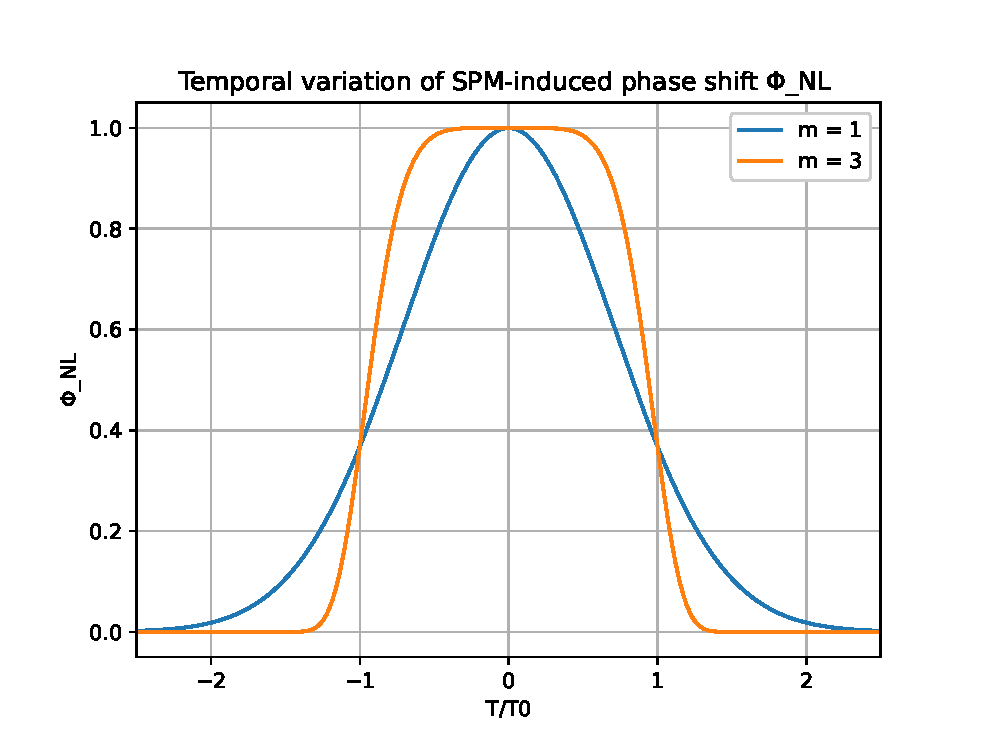
\includegraphics[width=1\textwidth]{figures/chap3/shift.eps}
            \caption{Phase shift $\phi_{NL}$.}
            \label{fig:shift_s}
        \end{subfigure}
        \hfill
        \begin{subfigure}[b]{.53\textwidth}
		    \centering	
            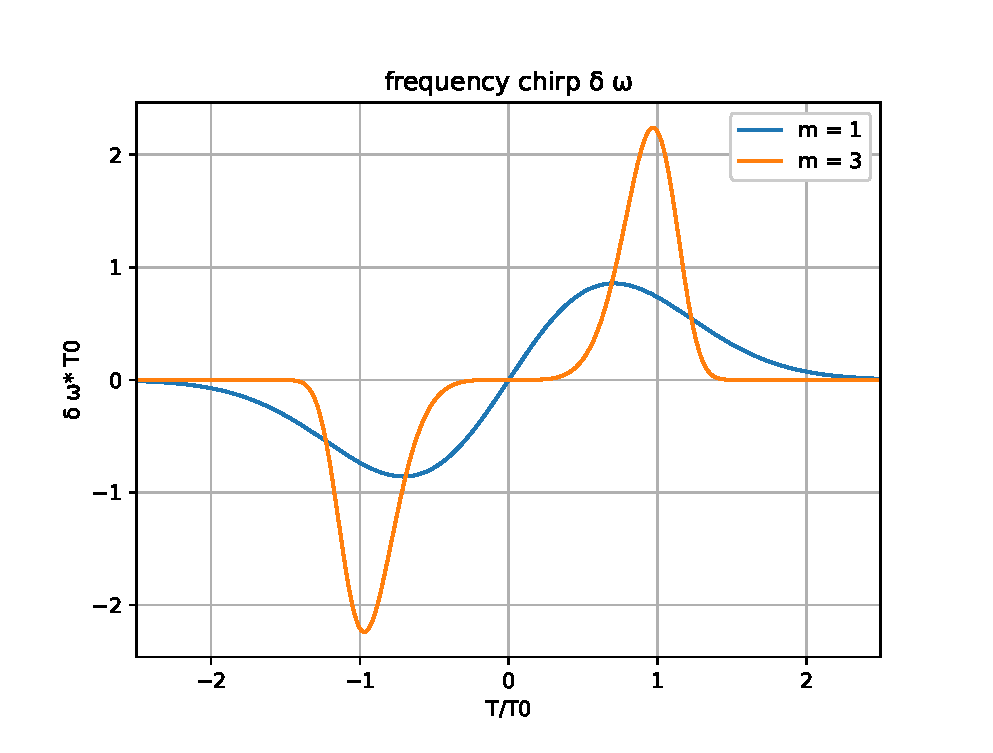
\includegraphics[width=1\textwidth]{figures/chap3/chirp.eps}
            \caption{Frequency chirp $\delta \omega$.}
            \label{fig:chirp_s}
        \end{subfigure}
        \end{tabular}
        \end{figure}
        
         \begin{figure}[label={fig:spmsech}, caption={Effect of SPM in a Sech pulse.}]
         \centering
        \begin{tabular}[c]{cc}
        \centering
        \begin{subfigure}[b]{.53\textwidth}
		    \centering	
            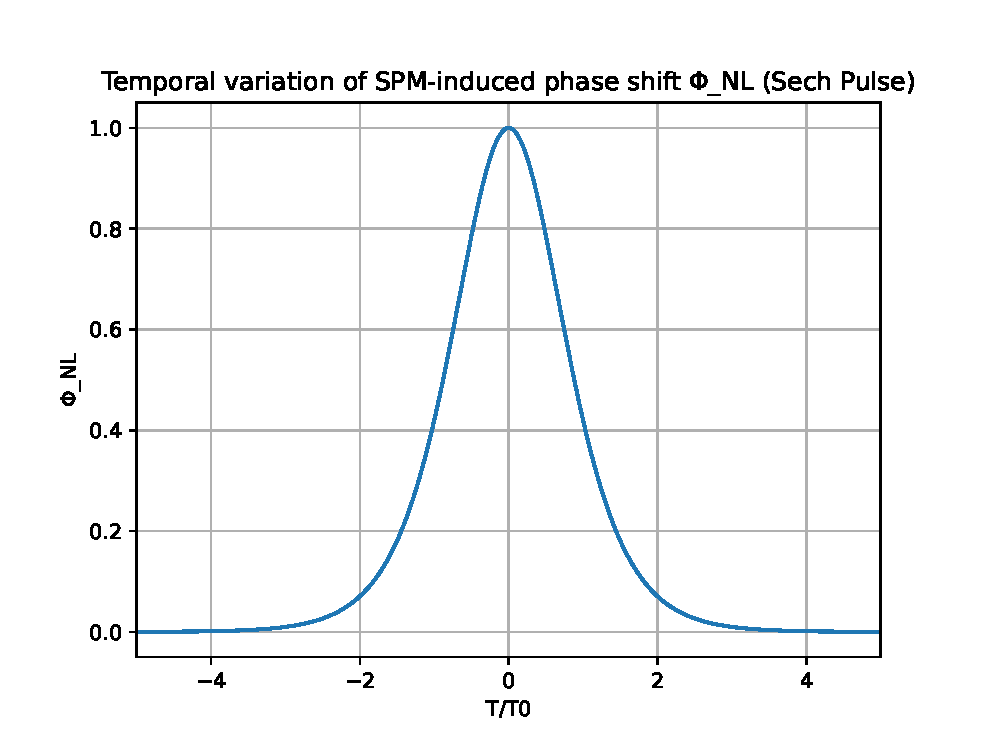
\includegraphics[width=1\textwidth]{figures/chap3/shift_sech.eps}
            \caption{Phase shift $\phi_{NL}$.}
            \label{fig:shift}
        \end{subfigure}
        \hfill
        \begin{subfigure}[b]{.53\textwidth}
		    \centering	
            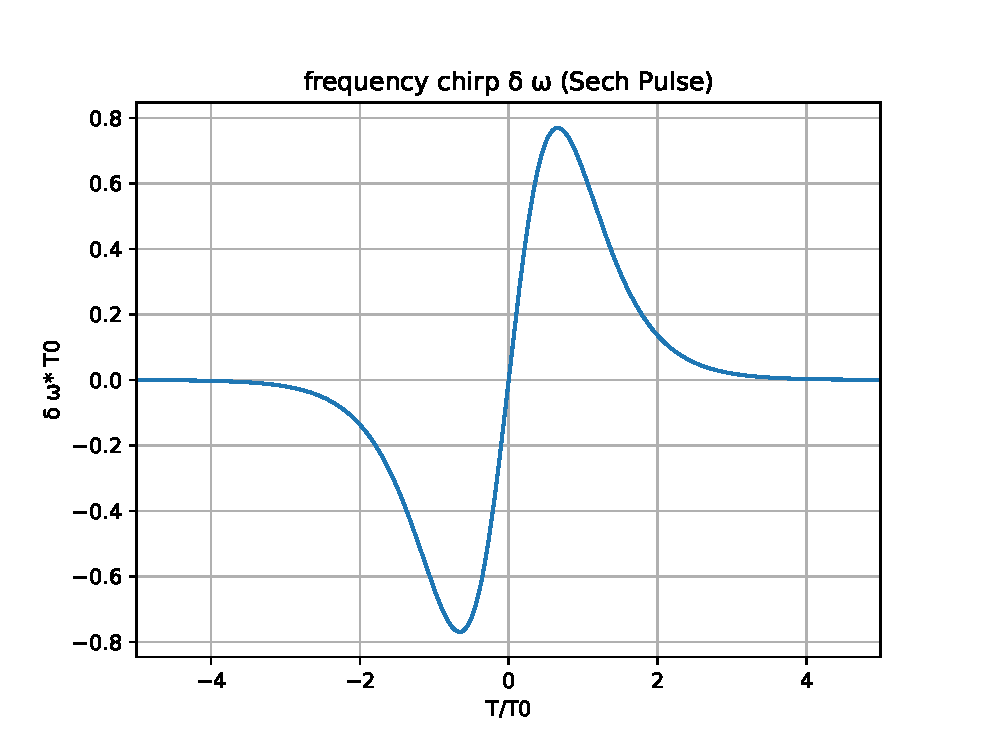
\includegraphics[width=1\textwidth]{figures/chap3/chirp_sech.eps}
            \caption{Frequency chirp $\delta \omega$.}
            \label{fig:chirp}
        \end{subfigure}
        \end{tabular}
        \end{figure}
        
        \subsection{Solution of the NLSE (SSFM)}\label{subsec:nlse}
            To initially solve the NLSE through the SSFM, the equations to follow are \eqref{eq_dpn}, \eqref{eq_dhat}, and \eqref{eq_nhat}. As the objective of this project is to create an interactive web tool with learning purposes, we avoided some calculations related to Raman Scattering and other nonlinear effects. Thus, equation \eqref{eq_nhat} turns out to be 
            \begin{equation} \label{eq_nhat2}
             \hat{\mathcal{N}} = i \left( 
             %\frac{e^{-\alpha z} \gamma P_0 T^2_0}{\left|\beta_2\right|} \left|U\right|^2 
             e^{-\alpha z} \gamma P_0 \left|U\right|^2 
             \right) \ ,
        \end{equation}
        
        and using equation \eqref{eq_A0} in \eqref{eq_dpn}, we obtain
        \begin{equation}\label{eq_dpn2}
            \frac{\partial U}{\partial z} = \left( \hat{\mathcal{D}} + \hat{\mathcal{N}} \right) U \ . 
        \end{equation}
        
        It is now reasonable to introduce the parameter N, whose integer values give the soliton order:
        
        \begin{equation}\label{eq_n}
            N^2 = \frac{L_D}{L_{NL}} = \frac{\gamma P_0 T^2_0 \ . }{\left|\beta_2\right|}
        \end{equation}
        
        
        Depending on the value of \emph{N}, the SPM or GVD effects are more significant through the fiber. Some examples are carried by Agrawal \citep{AgrawalBook} for N = 0 (No SPM) and N = 1, then we compared them against the results we obtained with our code (figures \ref{fig:n1pb} and \ref{fig:n1nb}). 
        
         \begin{figure}[label={fig:n1pb}, caption={Solution of the NLSE using SSFM for N=1 and $\beta_2 > 0$.}]
         \centering	
         \begin{tabular}[c]{cc}
         \centering	
        \begin{subfigure}[b]{.53\textwidth}
        \centering	
            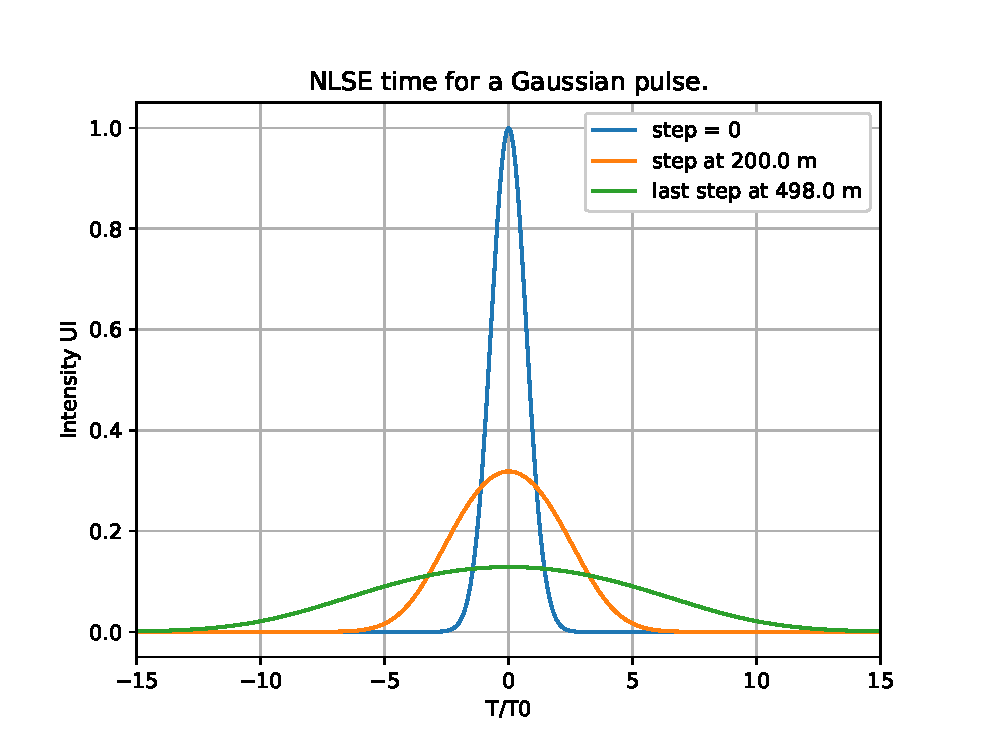
\includegraphics[width=1\textwidth]{figures/chap3/SSFM/eN1bt.eps}
            \caption{Envelope (time).}
            \label{fig:eN1bt}
        \end{subfigure}
        \begin{subfigure}[b]{.53\textwidth}
		    \centering	
            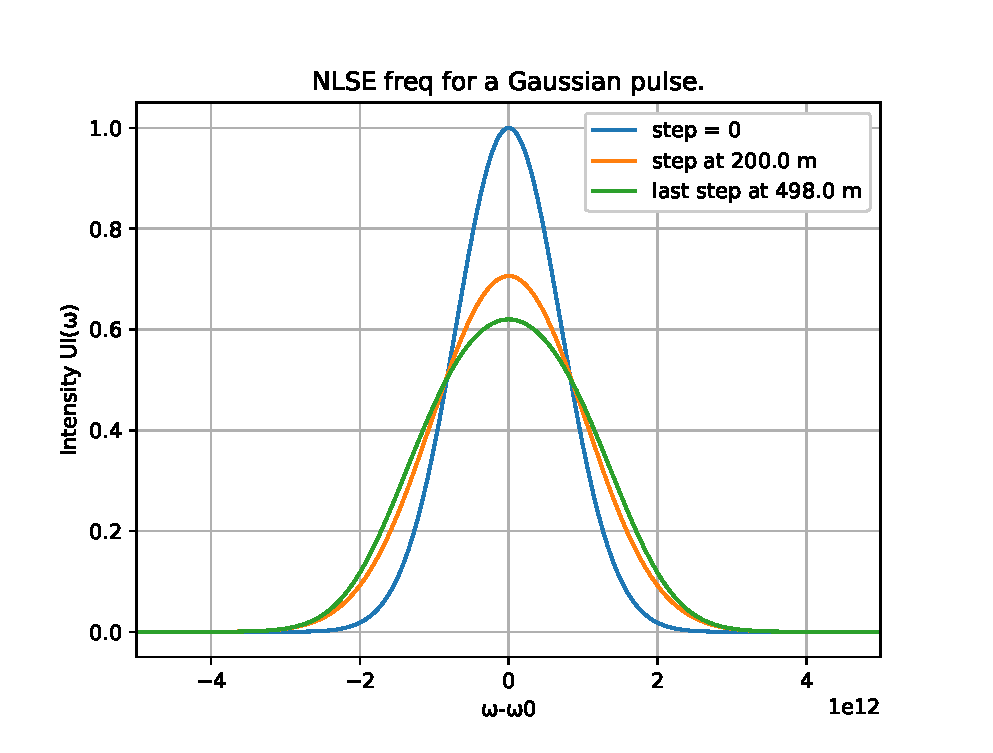
\includegraphics[width=1\textwidth]{figures/chap3/SSFM/eN1bs.eps}
            \caption{Envelope (spectrum).}
            \label{fig:eN1bs}
        \end{subfigure}
        \end{tabular}
        \begin{tabular}[c]{cc}
        \centering	
        \begin{subfigure}[b]{.53\textwidth}
		    \centering	
            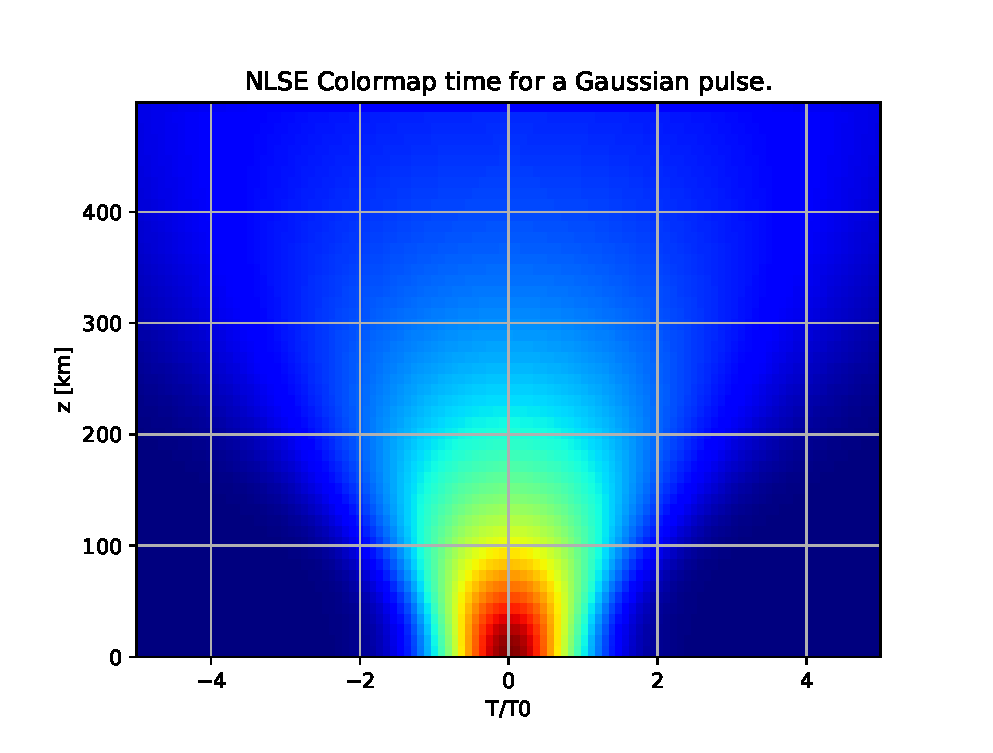
\includegraphics[width=1\textwidth]{figures/chap3/SSFM/N1bt.eps}
            \caption{Propagation (time).}
            \label{fig:N1bt}
        \end{subfigure}
        \hfill
        \begin{subfigure}[b]{.53\textwidth}
		    \centering	
            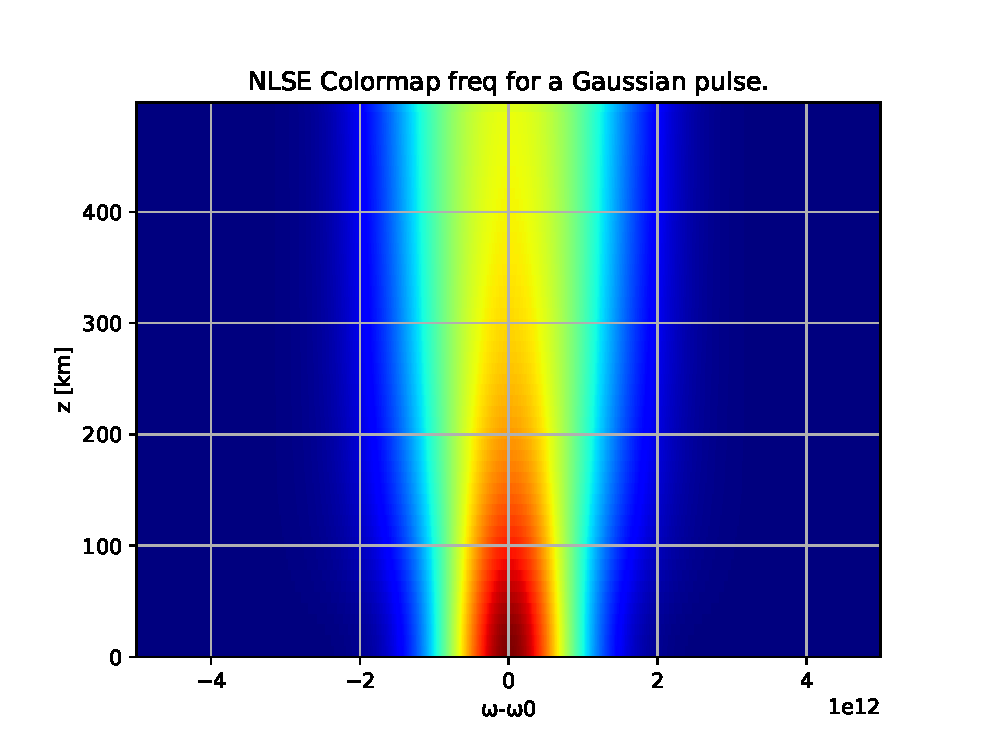
\includegraphics[width=1\textwidth]{figures/chap3/SSFM/N1bs.eps}
            \caption{Propagation (spectrum).}
            \label{fig:N1bs}
        \end{subfigure}
        \end{tabular}
        \end{figure}
        
         \begin{figure}[label={fig:n1nb}, caption={Solution of the NLSE using SSFM for N=1 and $\beta_2 < 0$.}]
         \centering	
         \begin{tabular}[c]{cc}
         \centering	
        \begin{subfigure}[b]{.53\textwidth}
		    \centering	
            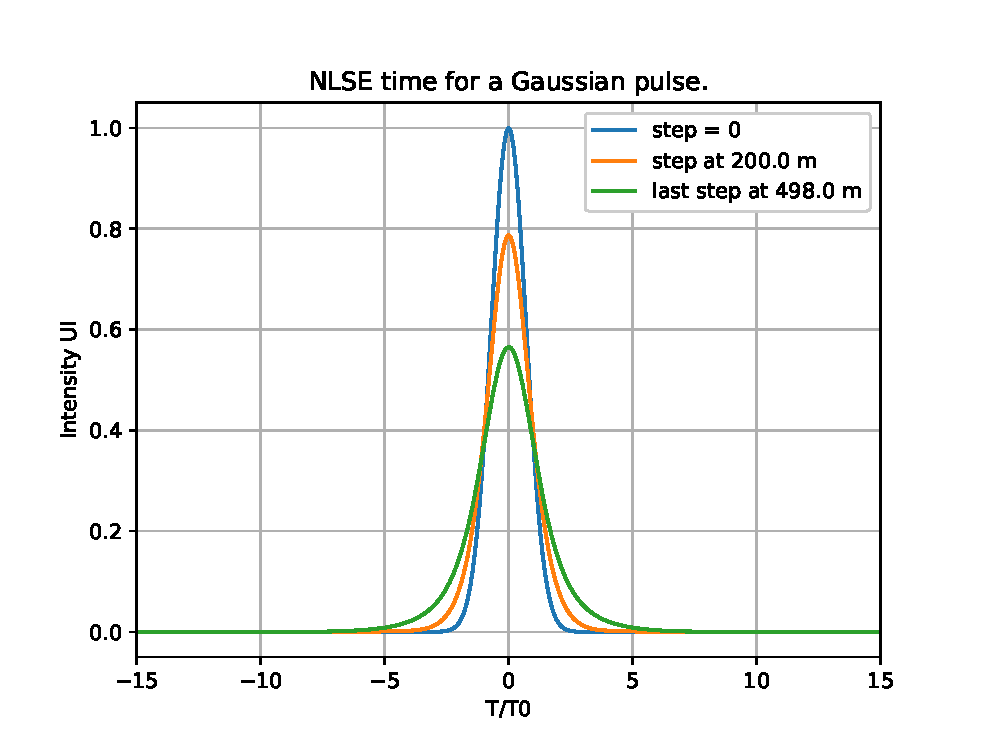
\includegraphics[width=1\linewidth]{figures/chap3/SSFM/eN1nbt.eps}
            \caption{Envelope (time).}
            \label{fig:eN1nbt}
        \end{subfigure}
        \hfill
        \begin{subfigure}[b]{.53\textwidth}
		    \centering	
            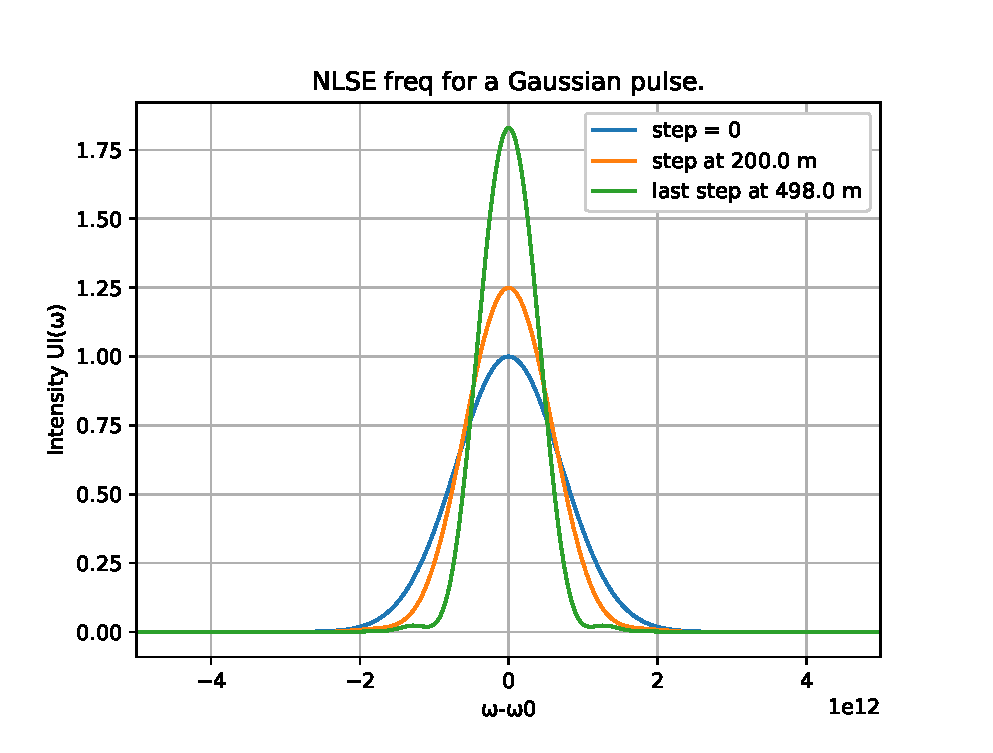
\includegraphics[width=1\linewidth]{figures/chap3/SSFM/eN1nbs.eps}
            \caption{Envelope (spectrum).}
            \label{fig:eN1nbs}
        \end{subfigure}
        \end{tabular}
        \begin{tabular}[c]{cc}
        \centering	
        \begin{subfigure}[b]{.53\textwidth}
		    \centering	
            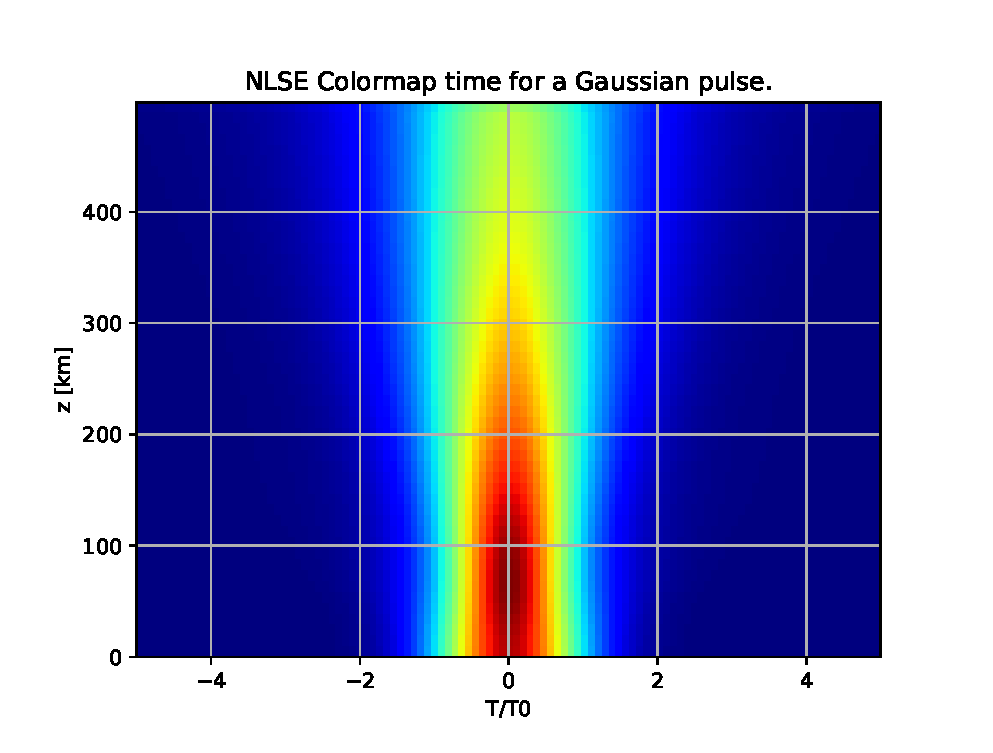
\includegraphics[width=1\linewidth]{figures/chap3/SSFM/N1nbt.eps}
            \caption{Propagation (time).}
            \label{fig:N1nbt}
        \end{subfigure}
        \hfill
        \begin{subfigure}[b]{.53\textwidth}
		    \centering	
            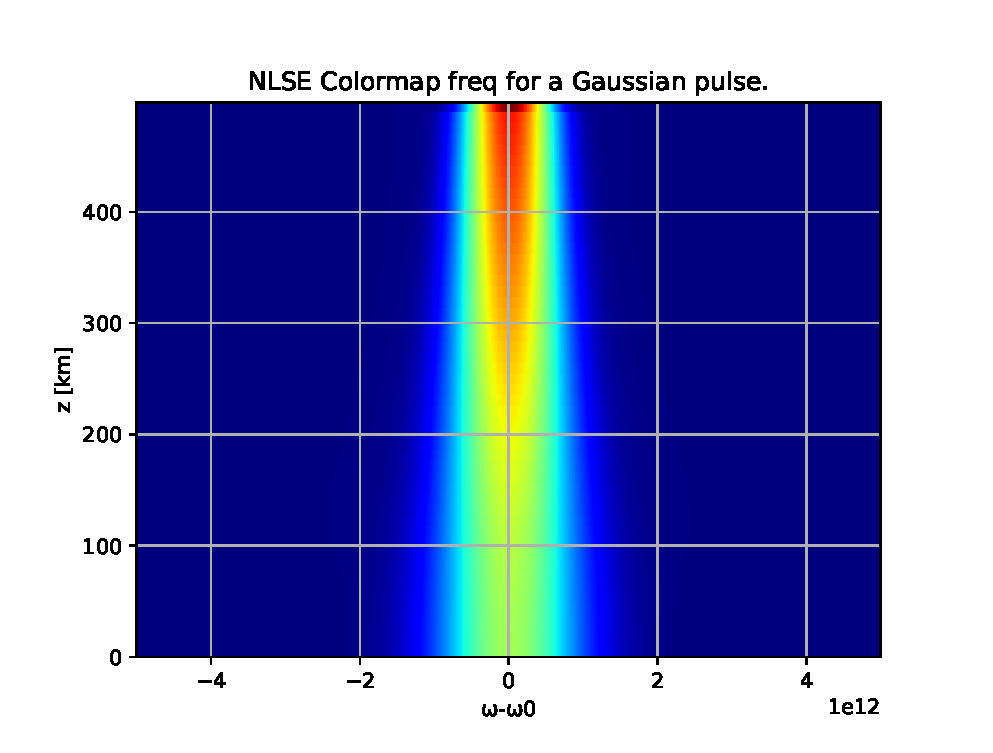
\includegraphics[width=1\linewidth]{figures/chap3/SSFM/N1nbs.eps}
            \caption{Propagation (spectrum).}
            \label{fig:N1nbs}
        \end{subfigure}
        \end{tabular}
        \end{figure}

    Following \citep{stolen}, the frequency spectra of a Gaussian pulse dependent on some values of maximum phase-shift is expected to be as given in figure \subref{fig:spmstol}. Figures \subref{fig:spm0pi}-\subref{fig:spm35pi} present the result of the function \emph{split\_step()} in the absence of dispersive effects (or close to the zero-dispersion region). The results of the code are very close to such shapes expected to get. The calculations were carried for a pulse $T_0 = 1ps$ in a lossless fiber with a length $L = 500m$, and $h = 0.004*L$ (250 steps).
    
     \begin{figure}[label={fig:spmssfm}, caption={Shape of the spectra for Gaussian pulses by maximum phase shift ($\phi_{NL}$).}]
         \centering	
         \begin{tabular}[c]{cc}
         \centering	
        \begin{subfigure}[b]{.53\textwidth}
		    \centering	
            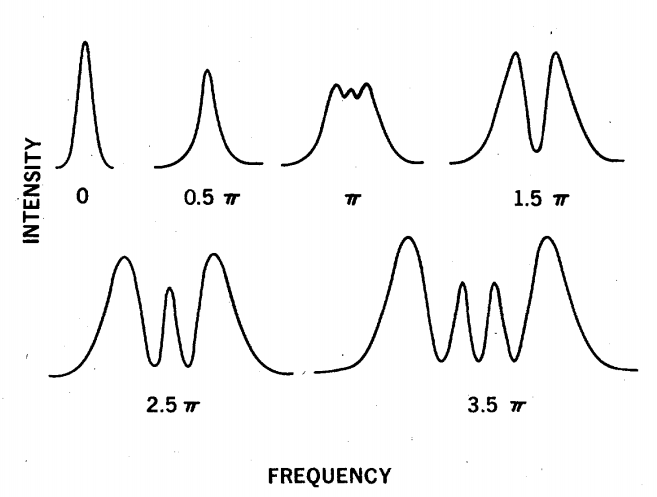
\includegraphics[width=1\linewidth]{figures/chap3/ssfm_spm/stolen_SPM.png}
            \caption{Calculated freq. spectra. Taken from \citep{stolen}}
            \label{fig:spmstol}
        \end{subfigure}
        \hfill
        \begin{subfigure}[b]{.53\textwidth}
		    \centering	
            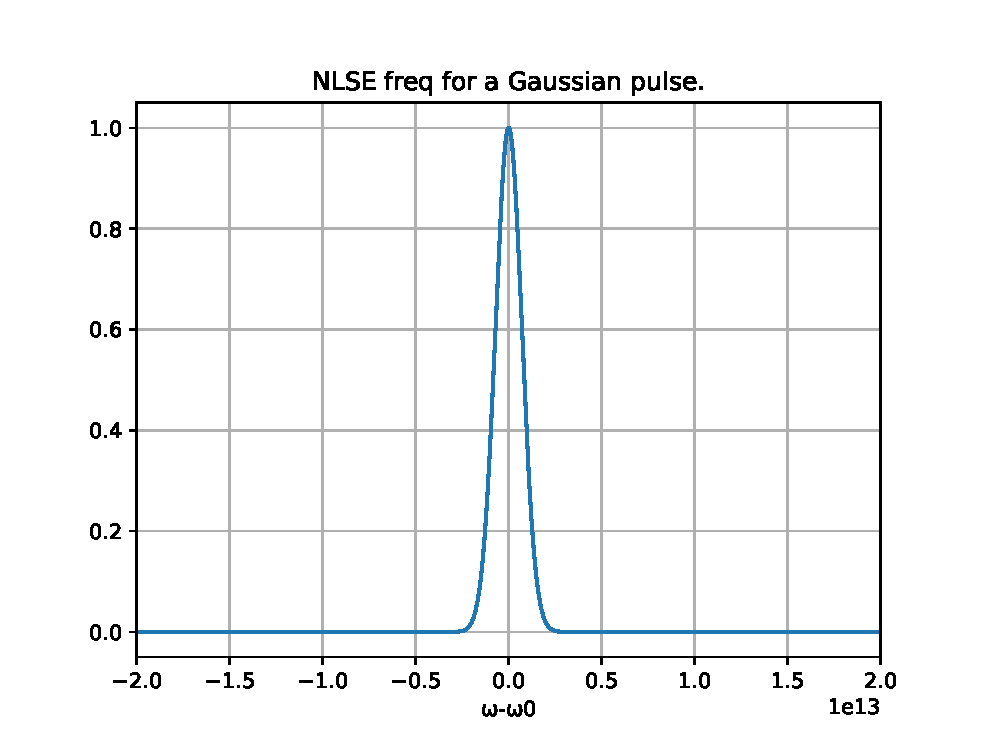
\includegraphics[width=1\linewidth]{figures/chap3/ssfm_spm/0pi.eps}
            \caption{$\phi_{NLmax}= 0$.}
            \label{fig:spm0pi}
        \end{subfigure}
        \end{tabular}
        \begin{tabular}[c]{cc}
        \begin{subfigure}[b]{.53\textwidth}
		    \centering	
            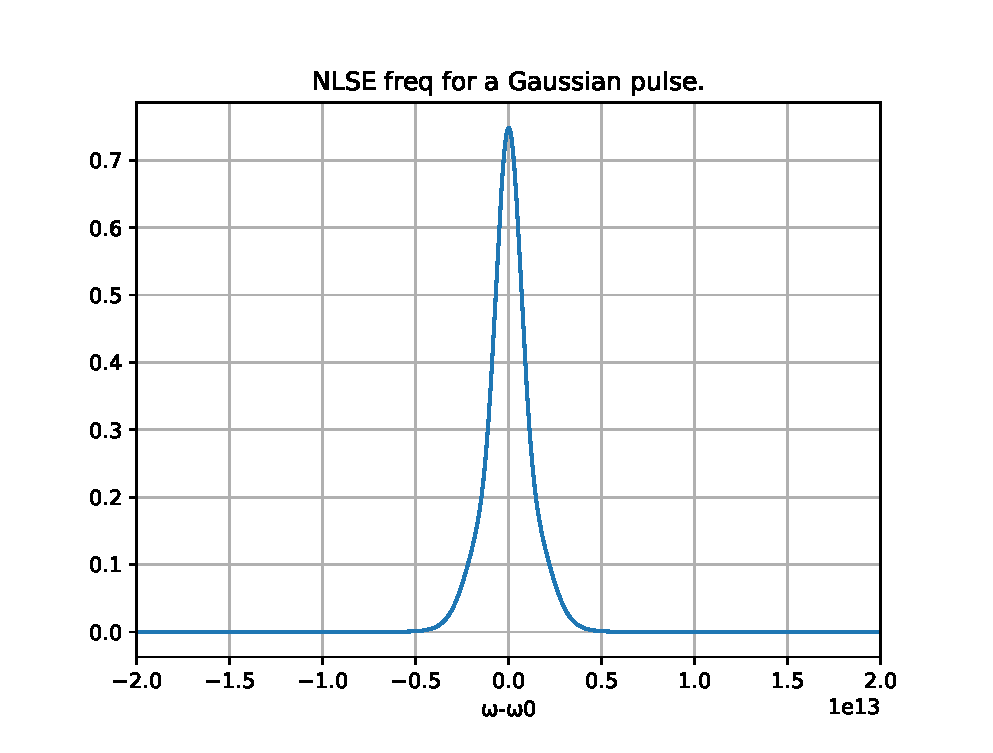
\includegraphics[width=1\linewidth]{figures/chap3/ssfm_spm/0_5pi.eps}
            \caption{$\phi_{NLmax}= 0.5\pi$.}
            \label{fig:spm05pi}
        \end{subfigure}
        \hfill
        \begin{subfigure}[b]{.53\textwidth}
		    \centering	
            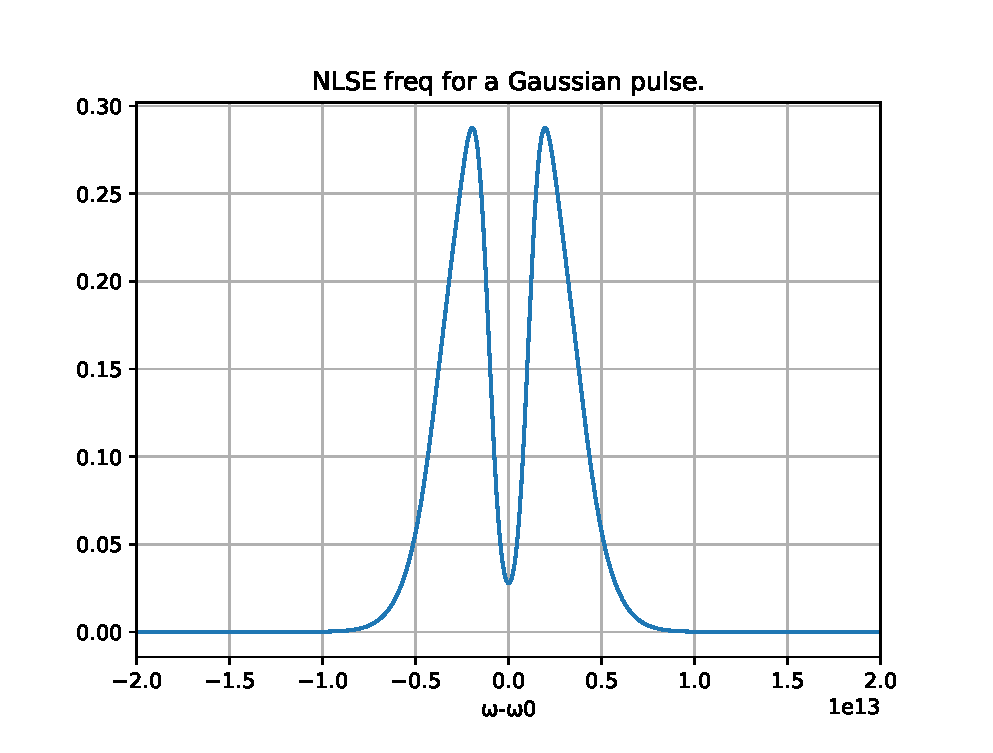
\includegraphics[width=1\linewidth]{figures/chap3/ssfm_spm/1_5pi.eps}
            \caption{$\phi_{NLmax}= 1.5\pi$.}
            \label{fig:spm15pi}
        \end{subfigure}
        \end{tabular}
        \begin{tabular}[c]{cc}
        \centering	
        \begin{subfigure}[b]{.53\textwidth}
		    \centering	
            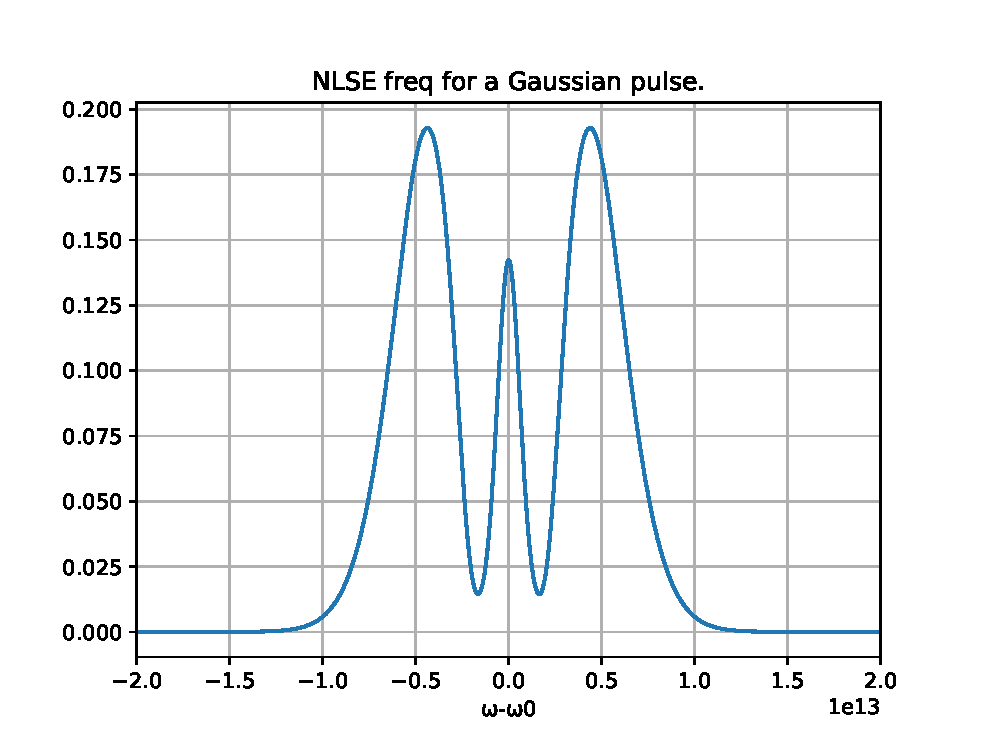
\includegraphics[width=1\linewidth]{figures/chap3/ssfm_spm/2_5pi.eps}
            \caption{$\phi_{NLmax}= 2.5\pi$.}
            \label{fig:spm25pi}
        \end{subfigure}
        \hfill
        \begin{subfigure}[b]{.53\textwidth}
		    \centering	
            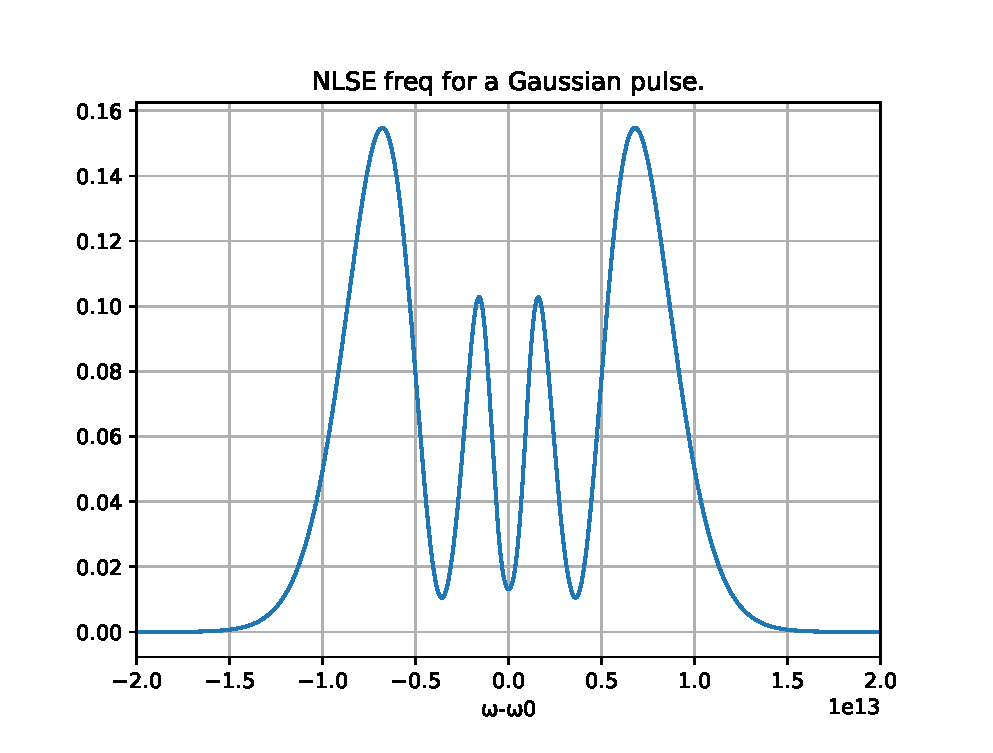
\includegraphics[width=1\linewidth]{figures/chap3/ssfm_spm/3_5pi.eps}
            \caption{$\phi_{NLmax}= 3.5\pi$.}
            \label{fig:spm35pi}
        \end{subfigure}
        \end{tabular}
        \end{figure}
    
    
    
\section{Web-Tool}
    Following the experience with the Fiber-mode App (previous chapter), Dash/Plotly works as a framework to build the web interface for the code written in Python. Other options such as Bokeh\footnote{\url{https://bokeh.org/}}  were considered, even though Dash did not present problems with some of the types of data used. In addition, it allows us to present intuitive and cleaner plots. 
    
    This open-source Python library has the advantage of providing a reactive app, which will allow the students (or general users) to use it on browsers regardless of the device and operative system, i.e., smartphones (Android, IOS, etc.), tablets, computers, etc. Thus, we implement the theories of interactive learning and strive to provide an online tool (additional to the lectures, books, and illustrations) to aid the students and, expectedly, motivate them to understand the effects involved in the propagation of short pulses on fibers. 
    The purpose of deploying this additional content online is to reach the necessities of most of the target population. Last year several universities around the globe had to do online teaching, and many activities of students' life migrated to the online aspect \citep{Hassel2020}. The average students possess (now more than ever) access to the internet, and, additionally, most of them have experience using online apps. Now, one can say that the app is accessible and flexible due to the previously mentioned characteristics. However, the intuitive part comes while developing the user interface. The application should help the user learn from it without vast information or 'how-to' tutorials. Consequently, it is crucial to place elements like buttons, sliders, or plots correctly. Figure \ref{fig:appdash} shows the global structure of the code. 
    
    \begin{figure}[label={fig:appdash}, caption={Global structure of the code.}]
          %  \caption*{Source: Some Source}
        	\includegraphics[trim = 0cm 0.5cm 0 1.2cm, clip, width=0.75\textwidth]{figures/chap3/Apps.eps} 
        \end{figure}
    
     The file init\_variables.py (Appendix \ref{sec:initvariables}) contains the necessary classes and functions to run all calculations needed for either the page or a local use with Matplotlib or directly Dash as localhost. Figure \ref{fig:UML} presents the class diagram of this file. 

    As inputs for the class Pulse, we have the pulse width T0, the time window T, the pulse type (either 'Gaussian' or 'Sech'), the initial chirp \textbf{C}, and, if necessary, the value of \textbf{m} for Super-Gaussian pulses. This class is in charge of initializing the pulse at z = 0. Then, the class Propagation receives the required inputs to solve the problem needed, i.e., it can return the solution for just GVD effects, just SPM effects (in this case, the phase shift and the frequency chirp), or the SSFM. One can also calculate the values of $L_D$, $L_{NL}$, $L_{eff}$, and $\phi_{NLmax}$. It is possible further to create Plotly's graphical objects essential to plot with Dash. This way, one can avoid writing more code lines while building the dash apps. 
    
    \begin{figure}[label={fig:UML}, caption={Class Diagram of init\_variables.py}]	\includegraphics[width=.6\textwidth]{figures/chap3/init_variables.eps} 
        \end{figure}
    
    \subsection{GVD code for python}
    The code responsible for providing the app for only dispersive effects to the user is the file \emph{gvd.py} (Appendix B). This code uses either 'only\_gvd' or 'gauss\_gvd' as solution type. The class is then in charge of using the methods previously mentioned in section \ref{subsect:gvd}. Sliders allow to change the values of $\beta_2$, initial chirp, m, and z, while a switch changes between Gaussian and Sech. In addition, the callbacks are always returning the actual state of the values along with the new calculated plots.  A simple block diagram of this page is presented in figure \ref{fig:gvddash}.
        
    \begin{figure}[label={fig:gvddash}, caption={Simplified Block-Diagram of gvd.py}]
          %  \caption*{Source: Some Source}
        	\includegraphics[trim = 2.5cm 12.5cm 5cm 2.5cm, clip, clip,width=1\textwidth]{figures/chap3/GVD.eps} 
        \end{figure}
    \subsection{SPM code for python}
    Figure \ref{fig:spmdash} bestows a simplified view of the SPM-page's structure.  The front-end receives values of $\gamma$, $P_0$, and m. Then, it shows the plots of phase shift and frequency chirp together with the actual value of $L_{NL}$. 
        \begin{figure}[label={fig:spmdash}, caption={Simplified Block-Diagram of spm.py}]
          %  \caption*{Source: Some Source}
        	\includegraphics[trim = 0.5cm 12.5cm 6.5cm 1.2cm, clip, clip,width=1\textwidth]{figures/chap3/SPM.eps} 
        \end{figure}
        
    \subsection{NLSE}
        As discussed in section \ref{subsec:nlse}, the SSFM plays a meaningful role in this app.  This page is more intricate than the previous two mentioned due to the complexity of its callbacks and the number of input variables. Again, its block diagram is in figure \ref{fig:ssfmdash}. 
        
        \begin{figure}[label={fig:ssfmdash}, caption={Simplified Block-Diagram of nlse.py}]
          %  \caption*{Source: Some Source}
        	\includegraphics[trim = 0.5cm 12.5cm 6.5cm 0.6cm, clip, clip,width=1\textwidth]{figures/chap3/SSFM.eps} 
        \end{figure}
		\chapter{Results}
\label{results}
    At the early stages of testing and debugging, the pulse class (called in the Dash's app to plot and update with the callbacks) had to be necessarily declared as global. The global definition of this variable allowed us to share the results of the propagation's computation with the callback in charge of plotting the envelope without needing to trigger a new calculation for each value of z. That means that we have to treat the pulse envelope's plots and the heatmaps separately to avoid slower interactions in the app. This use of global variables is very effective while working locally, even though it led to problems when the app is used on different devices or browsers, affecting the results of all users at the same time.

According to Dash's documentation\footnote{\href{https://dash.plotly.com/sharing-data-between-callbacks}{Sharing Data Between Callbacks}}, the information between callbacks can (and should) be carried by using the Store component. After implementing this fix on the app, tests using a local server with two devices (local machine using two different web-browsers and a smartphone) showed that the problem didn't persist. Figures \ref{fig:herokugvd} to \ref{fig:herokunlse} in Appendix \ref{Appendixapp} show the Dash layout. 

Each web app links the other two to connect the three previously discussed regimes divided by "GVD," "SPM," and "NLSE" apps. These applications were tested in a debugging mode to assure that they operate correctly and check their performance.  The right assignation of memory is then meaningful while using the Dash's Store component. For instance, the size of the variables stored locally shouldn't exceed 2MB for most of the environments (up to 10 MB for desktop webbrowsers), as stated by Plotly\footnote{\url{https://dash.plotly.com/dash-core-components/store}}. The arrays containing the data of the intensities in time and spectrum were selected to size approximately 0.813MB each, whose length is 13x8192 points. Besides, the array sampling the z values has a byte-size of 208B for 13 sampled points (taken from the 250 steps of the SSFM), which operates very fluently for local use. Subsequently, tests on an Android device, as well as on a computer, showed that the app is ready to deploy. We carried the examinations using Chrome, Firefox, and Edge on a laptop; and Chrome and Firefox on an Android device.

% SIZE:  1704056 1704056 312
% Size:  (26, 8192) (26, 8192) (26,)
% Type:  float64 float64 float64


% SIZE:  852088 852088 208
% Size:  (13, 8192) (13, 8192) (13,)
% Type:  float64 float64 float64


    \section{Deployment of the web-tool}
        \subsection{Heroku (Free servers)}
            Let us now turn our attention to the deployment of this app and its distribution to the final users. The first step is to test the app using a free service such as Heroku. Thereupon we set the git repository and structured the app following Dash's/Plotly's instructions\footnote{\url{https://dash.plotly.com/deployment}}. The deployment presented some problems concerning responsitivity and calculation time. In consequence, the number of steps for SSFM had to be downscaled from 250 to 100 points. Finally, the app (under the name of pulse\_app) was released using the European region and is located at the following link: \url{https://pulse-app-mpsp.herokuapp.com/apps/nlse}.
            
            The Dash environment allows printing the shown plots; besides, pushing the button "Download parameters as text" triggers a download of a '.txt' file containing all the parameters used at that exact point.
    
       
        
        
        
        \subsection{Max Planck School of Photonics' learning platform}
        During the assessment and definition of objectives for this thesis, we evaluated the possibility of hosting the final app in a platform such as the virtual campus of \gls{MPSP}. Despite this, after some research, we concluded that it is not possible to host or build a Python-based app directly on Moodle-like platforms such as the one previously mentioned. Nevertheless, it is possible to embed Python/Dash's layouts inside those services using the "src" attribute of HTML to post the app hosted in a service similar to Heroku.
         



\chapter{Conclusion}
    
    \section{Hosting the server}
    \section{Future work}
    
		%\chapter{Template Features}
This chapter gives examples on what you can do with this template. It's just a brief overview. Please consult the common sources on how to write scientific documents and documents with \LaTeX.

\section{Structure}
This template provides three structural levels that appear in the table of contents: \texttt{\textbackslash chapter}, \texttt{\textbackslash section}, and \texttt{\textbackslash subsection}. Chapters will always start on a new page. Additionally, you can use \texttt{\textbackslash subsubsection} and \texttt{\textbackslash paragraph} as non-hierarchical means to structure your thesis.


\subsection{Lists}
You can use the default \LaTeX \- functions for writing lists, viz., \texttt{\textbackslash enumerate} for numbered lists and \texttt{\textbackslash itemize} for bullet point lists. Again, the \texttt{\textbackslash subsubsection} and \texttt{\textbackslash paragraph} can be used as structural elements, e.g., when listing definitions of terms.

\subsection{Footnotes}
Footnotes are continuously numbered throughout the document. Use the \texttt{\textbackslash footnote\{text\}} command.  They appear on the page their reference is on \footnote{This is an exemplary footnote.}. Footnotes have to be placed without whitespace behind the word and within the sentence boundaries, i.e., before the period.

\subsection{ToDo-Notes}
You can use ToDo notes using the \texttt{\textbackslash todo\{text\}}  command. Please make sure to remove any ToDo notes before handing in your thesis! \todo[inline]{ToDo: Remove me before publishing}

\section{Formatting Text}
\LaTeX \- provides \texttt{\textbackslash textit\{text\}} for \textit{italics}, \texttt{\textbackslash textbf\{text\}} for \textbf{bold face}, \texttt{\textbackslash texttt\{text\}} for \texttt{typewriter}, \texttt{\textbackslash textsc\{text\}} for \textsc{small caps}, \texttt{\textbackslash underline\{text\}} for \underline{underline}. Additionally, the template provides  \texttt{\textbackslash texthl\{text\}} for \texthl{highlighted text}. Please remove any highlighted text before handing in your thesis!

Please use the \texttt{\textbackslash enquote\{text\}} command for \enquote{direct quotes}.

\subsection{Colors}
This template comes with the colors defined in the \gls{CD} of the \gls{FAU}. Table \ref{tab:colors} lists the color names. You can apply them to text by using the  \\ \texttt{\textbackslash textcolor\{color name\}\{text\}} command.
	
\begin{table}[caption={Colors defined by the template}, label=tab:colors]
	\centering
		\begin{tabular}{@{}ll@{}}
			\toprule
			{\bf Color Name} & {\bf Result} \\ \midrule
			fau-grey      & \textcolor{fau-grey}{Exemplary Text and 0123456789}  \\
			fau-red      & \textcolor{fau-red}{Exemplary Text and 0123456789}  \\
			fau-blue      & \textcolor{fau-blue}{Exemplary Text and 0123456789}  \\
			fau-cyan    & \textcolor{fau-cyan}{Exemplary Text and 0123456789}  \\
			fau-orange      & \textcolor{fau-orange}{Exemplary Text and 0123456789}  \\
			fau-green      & \textcolor{fau-green}{Exemplary Text and 0123456789}  \\ \midrule
		\end{tabular}
\end{table}


\section{Figures}

The \texttt{figure} environment is wrapped around images. These images should either be included as PDF-file via \texttt{\textbackslash includegraphics}, or created via \textit{TikZ/PGF}. For included images, make sure to use high-resolution images, preferably vector images.

Figures float, i.e., they do not necessarily appear at exact the same position you have defined them. Make sure to set a  \textit{caption} and an optional \textit{label} as figure parameters. 

\begin{figure}[label={fig:img01}, caption={Relationship of students and theses}]
  %  \caption*{Source: Some Source}
	
\includegraphics[width=.6\textwidth]{figures/figure01.pdf} 
\end{figure}


\subsection{Subfigures}
Sometimes it might be handy to contrast figures, i.e., by placing them next to each other. The template uses the \textit{subcaption} package to provide subfigures. The following example contains two figures, where each subfigure has its own \texttt{\textbackslash label} and \texttt{\textbackslash caption}. Additionally, the whole figure has its own \textit{caption} and \textit{label}. That means, you can reference subfigures  Figure \ref{fig:subfig1} and Figure  \ref{fig:subfig}. Only the whole figure will be listed in the table of figures.

Subfigures are not limited to images, but may also include listings or tables. Figure \ref{fig:subfig} shows a sample database query expressed in \gls{SQL} (Figure \ref{fig:subfig1}) and as query plan in relational algebra  (Figure \ref{fig:subfig2}).
 
\begin{figure}[caption={Exemplary use of subfigures}, label={fig:subfig}]
	
	\begin{subfigure}[b]{.45\textwidth}
		
		\begin{lstlisting}[nolol, language=SQL]
		SELECT b, d FROM 
			EXAMPLE.RELATION1 r,
			EXAMPLE.RELATION2 s,
		WHERE 
			r.a = 'c'
		AND 
			s.e = 2
		AND 
			r.c = s.c; 
		\end{lstlisting}
		\caption{\gls{SQL} select statement}\label{fig:subfig1}
	\end{subfigure}
	\begin{subfigure}[b]{.53\textwidth}
		\centering	
		\begin{tikzpicture}[node distance = 2cm, auto,
		database/.style={
			cylinder,
			cylinder uses custom fill,
			cylinder body fill=gray!30,
			cylinder end fill=gray!20,
			shape border rotate=90,
			aspect=0.25,
			draw
		}]
		\node [] (queue) {$\Pi_{b, d}$};
		\node [below of=queue] (join) {$\Join_{r.c = s.c}$};
		
		\node [below left of=join,xshift=-1cm] (l1) {$\sigma_{r.a = 'c'}$};
		\node [database, below of=l1] (l2) {\texttt{r}};
		
		\node [below right of=join,xshift=1cm] (r1) {$\sigma_{s.e = 2}$};
		\node [database,below of=r1] (r2) {\texttt{s}};
		
		\draw [<-] (queue) -- (join);
		\draw [<-] (join) -- (r1);
		\draw [<-] (r1) -- (r2);
		\draw [<-] (join) -- (l1);
		\draw [<-] (l1) -- (l2);
		\end{tikzpicture}
		\caption{Sample evaluation plan}\label{fig:subfig2}
	\end{subfigure}
\end{figure}
\section{Listings}
You can use listings to typeset source code. This template uses the \textit{listings} package. Wrap code inside the \texttt{lstlisting} environment and set the \textit{language} (e.g., Java, SQL), \textit{caption}, and optional \textit{label} parameters. If the source code highlighting highlights the wrong keywords or misses keywords, use the \textit{deletekeywords} resp. \textit{morekeywords} parameters. Consult the package documentation for further information.

\begin{lstlisting}[float=htp, caption={Euclid's GCD algorithm implemented in Java}, label={lst:euclid}, language=Java, deletekeywords={}, morekeywords={}]
public class Euclid {

	public static int gcd(int p, int q) {
		if (q == 0) return p;
		else return gcd(q, p % q);
	}

}
\end{lstlisting}

\section{Algorithms}
Some users might require specifying algorithms. This template uses the \textit{algorithm}, \textit{algorithmicx}, and \textit{algopseudocode} packages. Consult the respective manuals for further information. Algorithms do not appear in a table at the beginning of the document, i.e., there is no list of algorithms.

\begin{algorithm}[htb]
	\begin{algorithmic}
		\Require nonnegative integer $a$, nonnegative integer $b$
		\Function{Euclid}{$a, b$}
		\If {$b = 0$} \Comment{comment}
		\State{return $a$;}
		\Else 
		\State {return \textsc{Euclid}$(b, a\mod b)$;}
		\EndIf
		\EndFunction
	\end{algorithmic}
	\caption{Euclid's GCD algorithm in pseudocode}
	\label{alg:garbage}
\end{algorithm}

\section{Acronyms and Abbreviations}
This template provides comprehensive support for acronyms and abbreviations. The template uses the \textit{glossaries} package. 
Please do only define abbreviations and symbols that are uncommon. That means, common abbreviations such as \enquote{e.g.} or \enquote{i.e.} should not be listed. Abbreviations and symbols are sorted automatically by their label. 

\subsection{Custom Abbreviations}
Custom abbreviations are defined in the \path{config/acronyms.tex} file, using the \\
\texttt{\textbackslash newacronym[longplural=\{<long plural>\}, shortplural=\{<short plural>\}]\\ \{<label>\}\{<short>\}\{<long>\}} command. The \textit{longplural} and \textit{shortplural} parameters are optional. The abbreviations are sorted by their labels. The label is furthermore used to reference the abbreviations in your text. You can do so using commands listed in Table \ref{tab:glossaries}. In most cases, you just use \textbackslash gls\{<label>\}. On the first occurrence, the full version is displayed, e.g., \gls{diss}. Afterwards, the short version will be displayed, i.e., \gls{diss}.

You pluralize your abbreviation by adding a \texttt{pl} to a command. This will add a small s to the abbreviation, e.g., \glspl{diss}. Table \ref{tab:glossaries} shows custom short and long plural versions of the term and abbreviation \textquote{\gls{kmu}}. You might need this esp. for German abbreviations that do not have a \enquote{s} plural form.

\begin{table}[caption={Commands for printing abbreviations}, label=tab:glossaries]
	\centering
	\begin{tabular}{@{}ll@{}}
		\toprule
		{\bf Command} & {\bf Result} \\ \midrule
		\textbackslash gls\{<label>\}     & \textbackslash acrfull on first occurence, \textbackslash acrshort otherwise \\
		\textbackslash glspl\{<label>\}       &  \textbackslash acrfullpl on first occurence, \textbackslash acrshortpl otherwise \\
		\textbackslash acrshort\{<label>\}       & \acrshort{kmu} \\
		\textbackslash acrshortpl\{<label>\}       & \acrshortpl{kmu} \\
		\textbackslash acrlong\{<label>\}       & \acrlong{kmu} \\
		\textbackslash acrlongpl\{<label>\}      & \acrlongpl{kmu} \\
		\textbackslash acrfull\{<label>\}      & \acrfull{kmu} \\
		\textbackslash acrfullpl\{<label>\}     & \acrfullpl{kmu} \\ \bottomrule
	\end{tabular}
\end{table}

Only referenced abbreviations will be added to the list of abbreviations.

\subsection{Symbols}
If required, you can define symbols in the \path{symbols.tex} file, using the \\ \texttt{\textbackslash addsymboltolist\{<symbol>\}\{<label>\}\{<name>\}} command. The symbols are sorted by their labels. Please note, regardless of using the symbols in the text, all symbols defined in the symbols file will be output to the list of symbols.

\section{Citations and Bibliography}
This template uses {BibTeX} for bibliographies. It comes with the APA style that takes care of proper formatting and sorting of your references. Of course, you have to maintain a clean \path{library.bib} file that caters all necessary attributes. References will appear in the alphabetical order of the surname of the first author. In case of several works by the same author, they are sorted by year.

Citing in the text is done with the \textbackslash citep[<before>][<after>]\{<citekey>\} command. Citations without parenthesis are done with \textbackslash citet\{<citekey>\}.

\paragraph{Exemplary citations}

\begin{itemize}
	\item \gls{BPM} is an integral management paradigm for building and running effective and efficient organizations  \citep{Hammer2015, VomBrocke2014a}.
	\item A holistic approach to \gls{BPM} goes beyond process modeling and workflow management systems \citep[p.{530}]{VomBrocke2014a}.
	\item A conference citation \citep{Rozinat2008}.
	\item See \citet{VomBrocke2014a} for a comprehensive review on \gls{BPM} best practices.
	\item \citet{Hammer2015} lists organizational capabilities for \gls{BPM} \citep[cf.][pf.{9}]{Hammer2015}, while \citet[cf.][pp.{530--546}]{VomBrocke2014a} give principles of good \gls{BPM} .
	\item Two authors are automatically divided by an ampersand, e.g., \citep{Becker2011}.
	\item \enquote{\gls{BPM} can provide a solid set of capabilities essential to master contemporary and future challenges} \citep[p.{534}]{VomBrocke2014a}.
\end{itemize}


		
    \end{content}
    
    \pagenumbering{Roman}
    \setcounter{page}{\numexpr\value{savepage}}

    % References
    \references{}
    
    % Appendix
     \begin{appendix}
        % In the appendices, use \section{} instead of \chapter{}
         \section{Some Appendix Section}
\label{sec:appendix01}
Appendices provide only two structural levels, viz., \texttt{\textbackslash section}, and \texttt{\textbackslash subsection}.

The numbering of figures, listings, tables, and footnotes is not reset. Thus, it continues as usual in the appendix.

\subsection{Some Appendix Subsection}

\lipsum[10]
         \section{init\_variables.py}
\label{sec:initvariables}


\begin{minted}{python}
# coding:utf8
import numpy as np
import matplotlib.pyplot as plt
import dash_core_components as dcc
from scipy.integrate import cumtrapz, solve_ivp
import plotly.graph_objects as go
from numpy.core.numeric import Inf  


#Last edition date:
from datetime import date

from scipy.optimize import minpack
today = date.today()
date = today.strftime("%d.%m.%Y")###Edit before deployment with, e.g., '28.06.2021'
#-----------------//

##-----------NUMERICAL METHODS-----------##
#--------Derivatives--------#
def derivative(f,x0,method='central',dx=0.01):
    if method == 'central':
        return (f(x0 + dx) - f(x0 - dx))/(2*dx)
    elif method == 'forward':
        return (f(x0 + dx) - f(x0))/dx
    elif method == 'backward':
        return (f(x0) - f(x0 - dx))/dx
    else:
        raise ValueError("Method must be 'central', 'forward' or 'backward'.") #taken and edited from https://www.math.ubc.ca/~pwalls/math-python/differentiation/differentiation/
#--------------------------#
#----Mid-point Method------#
def mid_step(x0, f, T, *args):
    dt = T[1]-T[0]
    k = len(T)
    X = np.zeros(k)
    X[0]=x0
    for i in range(1,k,1):
        X[i] = X[i-1] + dt*f(T[i-1]+dt/2, *args)
    return X
#------------------------#
##------------------------------------##

##---------------------SPM---------------------##
#--frequency chirp for δω Gaussian Pulse--#
def delta_g(T, T_, Leff, LNL, m = 1):
    delta_w = ((2*m*Leff)/(T_*LNL))*((T/T_)**(2*m-1))*np.exp(-(T/T_)**(2*m)) #eq (4.1.9) Agrawal
    return delta_w
#-----------------------------------------#
##---------------------------------------------##

#--SPLIT STEP FUNCTIONS--#
def U_noGVD(z,val,gamma,P0,T0,alpha,beta2, beta3): 
    
    tempU = val
    # definition of f = N*U
    #f = 1j*(gamma*P0*T0**2/np.absolute(beta2))*(np.absolute(U)**2)*U
    #f = 1j*(np.exp(-alpha*z)*gamma*P0*T0**2)*(np.absolute(U)**2)*U
    '''
    dU(T,z)/dz = N*U(T,z) = i*exp(-alpha*z)/LNL*(|U(T,z)|²)*U(T,z)
    '''
    f  = 1j*(np.exp(-alpha*z)*gamma*P0)*(np.absolute(tempU)**2)*tempU
    return f
#--------------------CLASS--------------------------------#
class Pulse:
    def __init__(self,  T0, T,  m = 1, C=0, pulsetype = 'Gaussian', wavelength  = 1550E-9):
        self.pulsetype = pulsetype
        #self.solution_method = soltype
        self.wavelength = wavelength
        self.speed = 299792458
        self.w0 = (2*np.pi*self.speed)/(self.wavelength)
        self.T0 = T0
        self.T = T
        self.m = m
        if self.m == 0:
            self.m = 1
            print('m = 0 not allowed, working with 1 instead')
        self.C = C
        self.initParam()
        
        self.colors = { #Colors for the plots and web interface:
            'text': '#111111',
            'background': '#FFFFFF',
            'circle': 'whitesmoke',
            'even': 'darkgreen',
            'odd': 'darkblue',
            'other': 'darkred',
            }


    def initParam(self):
        self.dT = self.T[1]-self.T[0] # step_size
        self.points = len(self.T)
        #Normalized Slow-Varying Envelope
        if self.pulsetype == 'Gaussian':
            self.UT0 = (np.exp(-((1+1j*self.C)/2)*((self.T/self.T0)**(2*self.m)))).astype(complex) #dtype = 'complex' in order to have complex values on solve_ivp 
            # self.T_FWHM = 2*np.sqrt(np.log(2))*self.T0
            # self.T0 = self.T_FWHM
        elif self.pulsetype == 'Sech':
            self.UT0 = (1/(np.cosh(self.T/self.T0))*np.exp(-(1j*self.C*self.T**2)/(2*self.T0**2))).astype(complex)
            # self.T_FWHM = 2*np.log(1+np.sqrt(2))*self.T0
            # self.T0 = self.T_FWHM
        else:
            raise ValueError("Pulse '{0}' not found, it must be 'Sech' or 'Gaussian'.".format(self.pulsetype))
        self.UW0 =np.fft.fftshift(np.fft.ifft(self.UT0))
        self.W = 2*np.pi* np.fft.fftfreq(self.points, self.dT) #+ self.w0
        #2*pi*(-N/2:N/2-1)/(N*dT)
        self.W = np.fft.fftshift(self.W) 

#------------------------------------------------------------#


#------------------------CLASS-------------------------------#
class Propagation(Pulse):
    def __init__(self,T0, T, solve_type= 'incident_field', L=0.1, beta2=0, gamma=0, P0=0,  beta3=0, loss = 0, pulsetype = 'Gaussian', m = 1, C=0, z0=0,h_step = 0.004, size_array = 51, wavelength=1550E-9):
        Pulse.__init__(self, T0, T, m=m, C=C, pulsetype=pulsetype)
        self.wavelength = wavelength
        self.speed = 299792458
        self.w0 = (2*np.pi*self.speed)/(self.wavelength)
        self.zmax = L #[m]  #Max distance that will be evaluated
        self.beta2 = beta2 #[ps²/m]
        self.gamma = gamma #[1/(W m)] !!!!!! 
        self.P0 = P0 #[W]
        self.beta3= beta3 #[ps³/m]
        self.loss = loss*1E-3 #[dB/m]
        self.z0 = z0 #At this point will be evaluated the pulse while using the 'only_gvd' mode
        self.h_step = h_step #step-size of the SSFM
        self.size_array = size_array #Size of the array where we are going to save the values of U(T) and U(w)
        self.U = np.zeros((self.size_array,self.points), dtype=complex) # U(z,T) is divided by certain ammount of steps and it's time length is N for each one of the steps
        self.UW = np.zeros((self.size_array,self.points), dtype=complex)
        self.solve_type = solve_type

        if self.solve_type == 'only_gvd':
            self.incident_field()
        elif self.solve_type == 'gauss_gvd':
            self.Gaussian_pulse_GVD()
        elif self.solve_type == 'only_spm':
            self.incident_field_spm()
        elif self.solve_type == 'split_step':
            if self.beta2  == 0 or self.gamma  == 0 or self.P0 == 0:
                print('Either beta2, gamma or P0 are zero, this could lead to problems with the calculation of the current method selected!')
            if self.zmax  == 0:
                raise ValueError('Fiber Length cannot be 0 for de desired solution')       
            self.split_step()
        else:
            raise ValueError("Solution method '{0}' does not exist, it must be 'only_gvd', 'gauss_gvd','only_spm' or 'split_step'.".format(self.solve_type))

    #Lengths
    def compute_LD(self):#Dispersion Length:
        if self.beta2 != 0:
            return ((self.T0)**2)/np.absolute(self.beta2)
        else:
            return Inf 

    def compute_LNL(self):#Length for nonlinearities:
        if self.gamma != 0 and self.P0 != 0 :
            return 1/(self.gamma*self.P0)
        else:
            return Inf 

    def compute_Leff(self): #Effective Length:
        if self.alpha !=0:
            return (1 - np.exp(-self.alpha*self.zmax))/self.alpha
        else: 
            return self.zmax 

    def compute_phimax_nogvd(self):
        Leff = self.compute_Leff()
        return self.gamma*self.P0*Leff #####BE CAREFUL!!!!!!!!!!! 0*inf...

    ##------------------------For GVD------------------------##
    def incident_field(self):  #Function using Eq. 3.2.5 and 3.2.6
        self.UW = self.UW0*np.exp((1j*self.beta2*self.W**2*self.z0/2))
        self.UT = np.fft.fft(np.fft.fftshift(self.UW))
        self.UI = np.absolute(self.UT)**2
        self.UIW = np.absolute(self.UW)**2
        self.UIW = self.UIW/np.amax(self.UIW) 
        return self.UT, self.UI, self.UW, self.UIW

    def Gaussian_pulse_GVD(self): #Function using Eq. 3.2.7 and 3.2.9 Agrawal
        self.UT = self.T0/(np.sqrt(self.T0**2 - 1j*self.beta2*self.z0))*np.exp(-self.T**2/(2*(self.T0**2 - 1j*self.beta2*self.z0)))
        self.UI = np.absolute(self.UT)**2
        self.UW = np.fft.fftshift(np.fft.ifft(self.UT))
        self.UIW = np.absolute(self.UW)**2
        self.UIW = self.UIW/np.amax(self.UIW) 
        return self.UT, self.UI, self.UW, self.UIW


    def Sech_pulse_GVD(self):#Not used 
        self.U0 = 1/(np.cosh(self.T/self.T0))*np.exp(-(1j*self.C*self.T**2)/(2*self.T0**2))
        self.UT = self.T0/(np.sqrt(self.T0**2 - 1j*self.beta2*self.z0))*np.exp(-self.T**2/(2*(self.T0**2 - 1j*self.beta2*self.z0)))
        self.UI = np.absolute(self.UT)**2
        self.UW = np.fft.fftshift(np.fft.ifft(self.UT))
        self.UIW = np.absolute(self.UW)**2
        self.UIW = self.UIW/np.amax(self.UIW) 
        return self.UT, self.UI, self.UW, self.UIW
    ##-------------------------------------------------------##
    ##-------------------------------------------------------##


    ##------------------------For SPM------------------------##
    def incident_field_spm(self):
        #Leff = self.compute_Leff()
        LNL = self.compute_LNL()
        Leff = LNL # Normalized to get the plots from the book
        if self.pulsetype == 'Gaussian':
            if self.m <= 1: #This conditionals were written when the UT0 was not already generalized for chirped-super-gaussian pulsetypes. Following also the book Arawal
                self.Phi_NL = (Leff/LNL)*np.absolute(self.UT0)**2
                self.delta_w = delta_g(self.T, self.T0, Leff, LNL)
            else: 
                self.delta_w = delta_g(self.T, self.T0, Leff, LNL, self.m)
                #for array-like data
                #Phi_NL = -cumtrapz(delta_w, T, initial=0) #Default 'initial' is None, which means no value at x[0] 
                #for function-like input:
                self.Phi_NL = -mid_step(0, delta_g, self.T, self.T0, Leff, LNL, self.m)

        elif self.pulsetype == 'Sech':
            phinl = lambda t: (Leff/LNL)*np.absolute(1/(np.cosh(t/self.T0))*np.exp(-(1j*self.C*t**2)/(2*self.T0**2)))**2
            self.Phi_NL = phinl(self.T)
            self.delta_w = -derivative(phinl, self.T, dx=self.dT)
        else:
            raise ValueError("Pulse '{0}' not found, it must be 'Sech' or 'Gaussian'.".format(self.pulsetype))

        return self.Phi_NL, self.delta_w
    ##-------------------------------------------------------##
    ##-------------------------------------------------------##

    ##---------------------SPLIT-STEP------------------------##
    def split_step(self):
        self.alpha = np.log(10**(self.loss/10)) #log y = ln y / ln 10 
        h = self.zmax*self.h_step #step size m -> depends on how long is the fiber we are working with
        print('\nZ max.: ',self.zmax, 'm')
        print('h size: ',h, 'm')
        print('LD: ',self.compute_LD(), 'm')
        print('LNL: ',self.compute_LNL(), 'm')
        print('N = sqrt(LD/LNL) = : ',np.sqrt(self.compute_LD()/self.compute_LNL()))
        print(1/self.h_step,'number of points evaluated')
        #initial values for split-step
        self.U[0] = self.UT0  #first value for U(0,T)  
        self.UW[0] = self.UW0 #first value for U(0,W)  
        #for general def (Eq. (2.4.3)): 
        Dw = -(1j*self.beta2/2)*(1j*self.W)**2 + (self.beta3/6)*(1j*self.W)**3 - self.alpha/2 #D = -1j*beta2/2*(δ²/T²) + beta3/6*(δ³/T³) - alpha/2
        #TODO: create a way to extract the betas from an array and take them to the frequency domain
        self.z = np.zeros((self.size_array))#array for saving the nth-point U(T,zn) and U(w,zn)
        mi = int(1/(self.size_array*self.h_step)) #just a counter 
        j = 1
        Utemp = self.UT0[:] #variable to update

        #for i in np.linspace(1,zmax*1000-h,k):  if we pre-defined the resolution (or ammount of steps k) independent of the step size h
        for k in range(0,int(1/self.h_step),1): # from z to z+h k times until z_max is reached
            ztemp = k*h #  [m] actual z to evaluate
            Uwtemp = np.fft.fftshift(np.fft.ifft(Utemp))
            Utemp = np.fft.fft(np.fft.fftshift(np.exp((h/2)*Dw)*Uwtemp))
            sol = solve_ivp (U_noGVD, # function to integrate
                        (ztemp, ztemp+h) , # duration [ z_init - z_end ]
                        Utemp, # initial conditions
                        method ='RK23', # method of integration 23
                        #t_eval =np.linspace(z, z+h, size_array), # points where the sol. is stored
                        rtol =1e-8 , # relative accuracy
                        args =[self.gamma, self.P0, self.T0, self.alpha, self.beta2, self.beta3]) # arguments for the function
            Utemp = sol.y.T[-1] #value at z+h
            Uwtemp = np.fft.fftshift(np.fft.ifft(Utemp))
            Utemp = np.fft.fft(np.fft.fftshift(np.exp((h/2)*Dw)*Uwtemp))
            Uwtemp = np.fft.fftshift(np.fft.ifft(Utemp))
            if k == mi and j< self.size_array:
                self.z[j] = ztemp
                self.U[j] = Utemp
                self.UW[j] = Uwtemp
                j +=1 #for the next step
                mi += int(1/(self.size_array*self.h_step))
        self.z[-1] = ztemp
        self.U[-1] = Utemp
        self.UW[-1] = Uwtemp
        self.UI = np.absolute(self.U)**2
        self.UIW = np.absolute(self.UW)**2
        #self.UIW = self.UIW/np.amax(self.UIW) 
        self.UIW = self.UIW/np.amax(self.UIW[0])
        print('last z evaluated: ',ztemp, 'm')
        print('last z saved: ',self.z[-1], 'm')
        print('\u03B1 = {0}'.format('%.3f' % (self.alpha)))
        print('Leff = {0}'.format('%.3f' % (self.compute_Leff())))
        print('\u03C6 max = {0}*\u03C0'.format('%.3f' % (self.compute_phimax_nogvd()/np.pi)))
        #self.W += self.w0  #Change axis of the functions plot_propagation() and plot_envelope()
        return self.U, self.UI, self.UW, self.UIW, self.W, self.z

    ##-------------------------------------------------------##
    #----- PLOTS -----#
    def plot_propagation(self, mode = 'time', xrange = [-8, 8], size_img = 600):
        if mode == 'time':
            intensity = self.UI
            x = self.T/self.T0#np.sort(t),
            x_title = 'T/T0'
            #updatemenus = []
        elif mode == 'spectrum':
            intensity = self.UIW
            x = self.W
            x_title = '\u03C9-\u03C90'
            xrange = [-0.1E14, 0.1E14]
            # xrange = [-0.1E14+self.w0, 0.1E14+self.w0]
            # updatemenus = [
            #                 dict(
            #                     type="buttons",
            #                     direction="left",
            #                     buttons=list([
            #                         dict(
            #                             args=[{'xaxis.type': 'linear'}],
            #                             label="Linear Scale",
            #                             method="relayout"
            #                         ),
            #                         dict(
            #                             args=[{'xaxis.type': 'log'}],
            #                             label="Log Scale",
            #                             method="relayout"
            #                         )
            #                     ])
            #                 ),
            #             ]
        else:
            raise ValueError("Mode '{0}' not found. Modes available 'time' or 'spectrum'.".format(mode) )
        propagation = go.Figure(data=[go.Heatmap(
                    x = x,
                    y = self.z,#np.sort(z),
                    z = intensity,
                    #type = 'heatmap',
                    zsmooth = "best",#to avoid line at the end of the plot
                    colorscale = 'Jet')])
        propagation.update_layout(
                                width=size_img, height=size_img,
                                yaxis=dict(range=[self.z[0], self.z[-1]],title='z [m]', ), 
                                #xaxis=dict(title=x_title,), 
                                xaxis=dict(range=xrange,title=x_title,), 
                                )
        #propagation.update_layout(updatemenus=updatemenus)
        return propagation
#------------------------------------------------------------#
    def plot_envelope(self, mode = 'time', z0 = 0, xrange = [-8, 8],  yrange = [0, 1.1], size_img = 600):
        if mode == 'time':
            intensity = self.UI
            x = self.T/self.T0
            x_title = 'T/T0'
            y_title = '|U(z,T)|^2'
            #updatemenus = []
        elif mode == 'spectrum':
            intensity = self.UIW
            x = self.W
            x_title = '\u03C9-\u03C90'
            y_title = '|U(z,\u03C9)|^2'
            xrange = [-0.1E14, 0.1E14]
            # xrange = [-0.1E14+self.w0, 0.1E14+self.w0]
            # updatemenus = [
            #                 dict(
            #                     type="buttons",
            #                     direction="left",
            #                     buttons=list([
            #                         dict(
            #                             args=[{'xaxis.type': 'linear'}],
            #                             label="Linear Scale",
            #                             method="relayout"
            #                         ),
            #                         dict(
            #                             args=[{'xaxis.type': 'log'}],
            #                             label="Log Scale",
            #                             method="relayout"
            #                         )
            #                     ])
            #                 ),
            #             ]
        else:
            raise ValueError("Mode '{0}' not found. Modes available 'time' or 'spectrum'.".format(mode) )
        

        scatter = go.Scatter(x=x,y=intensity[z0], name = self.pulsetype,
                                line=dict(color=self.colors['even']))
        
        figure = go.Figure(data=[scatter]).update_layout(
                                width=size_img, height=size_img,
                                plot_bgcolor  = self.colors['background'],
                                paper_bgcolor = self.colors['background'],
                                font= {'color': self.colors['text']},
                                yaxis=dict(range=yrange,title=y_title, ), 
                                #axis=dict(title=x_title,), 
                                xaxis=dict(range=xrange,title=x_title, ), 
                                title = '{0} pulse.'.format(self.pulsetype),
                                )
        #figure.update_layout(updatemenus=updatemenus)
        return figure
        # To plot and prepare the go.Figure for use inside the call back, the object Pulse should be called:

        # env_fig = pulse.plot_envelope()
        # env_graph = dcc.Graph(id='desired_id', #id for callback purposes
        #                         animate=True,
        #                         figure=env_fig.update_layout(
        # ))        

    def plot_envelope_GVD(self, mode = 'time', xrange = [-8, 8],  yrange = [0, 1.1], size_img = 600, color = 'darkgreen' ):
        if mode == 'time':
            intensity = self.UI
            x = self.T/self.T0
            x_title = 'T/T0'
            y_title = '|U(z,T)|^2'
        elif mode == 'spectrum':
            intensity = self.UIW
            x = self.W
            x_title = '\u03C9-\u03C90'
            y_title = '|U(z,\u03C9)|^2'
            xrange = [-0.1E14, 0.1E14]
        else:
            raise ValueError("Mode '{0}' not found. Modes available 'time' or 'spectrum'.".format(mode) )
        

        scatter = go.Scatter(x=x,y=intensity, name = self.pulsetype,
                                line=dict(color=color))
        
        return go.Figure(data=[scatter]).update_layout(
                                width=size_img, height=size_img,
                                plot_bgcolor  = self.colors['background'],
                                paper_bgcolor = self.colors['background'],
                                font= {'color': self.colors['text']},
                                yaxis=dict(range=yrange,title=y_title, ), 
                                #xaxis=dict(title=x_title,), 
                                xaxis=dict(range=xrange,title=x_title, ), 
                                #title = '{0} pulse.'.format(self.pulsetype),
                                )
def plot_shift(pulse1, pulse2, pulse3, xrange = [-2.5, 2.5], yrange = [0, 1.1], size_img = 600):
    p1 = go.Scatter(x=pulse1.T/pulse1.T0 ,y=pulse1.Phi_NL, name = 'Gaussian',
                         line=dict(color='darkgreen'))

    p2 = go.Scatter(x=pulse2.T/pulse2.T0 ,y=pulse2.Phi_NL, name = 'Super-Gaussian',
                        line=dict(color='darkblue'))

    p3 = go.Scatter(x=pulse3.T/pulse3.T0 ,y=pulse3.Phi_NL, name = 'Sech',
                         line=dict(color='darkred'))

    spm_phase = go.Figure(data=[p1,p2,p3]).update_layout( 
        updatemenus = list([
            dict(
                type="buttons",
                active=0,
                buttons=list([   
                    dict(label = 'Gaussian',
                        method = 'update',
                        args = [{'visible': [True, True, False]},
                                {'title': 'Phase: Gaussian Pulse.'}]), 

                    dict(label = 'Sech',
                        method = 'update',
                        args = [{'visible': [False, False, True]},
                                {'title': '''
                                Phase: Sech Pulse.'''}])  
                ]),
            )
        ])
    )


    spm_phase.update_layout( 
                            width=size_img, height=size_img,
                            plot_bgcolor  = '#FFFFFF',
                            paper_bgcolor = '#FFFFFF',
                            font= {
                                    'color': '#111111'},
                            yaxis=dict(range=yrange,title='Phase \u03C6NL', 
                                        ), 
                            xaxis=dict(range=xrange,title='T/T0', 
                                        ), 
                            )
    return spm_phase


def plot_chirp(pulse1, pulse2, pulse3, xrange = [-2.5, 2.5], yrange = [-3, 3], size_img = 600):

    chirp1 = go.Scatter(x=pulse1.T/pulse1.T0 ,y=pulse1.delta_w*pulse1.T0, name = 'Gaussian',
                            line=dict(color='darkgreen'))
    
    chirp2 = go.Scatter(x=pulse2.T/pulse2.T0 ,y=pulse2.delta_w*pulse2.T0, name = 'Super-Gaussian',
                            line=dict(color='darkblue'))

    chirp3 = go.Scatter(x=pulse3.T/pulse3.T0 ,y=pulse3.delta_w*pulse3.T0, name = 'Sech',
                            line=dict(color='darkred'))


    spm_chirp = go.Figure(data=[chirp1,chirp2, chirp3]).update_layout( 
        updatemenus = list([
            dict(
                type="buttons",
                active=0,
                buttons=list([   
                    dict(label = 'Gaussian',
                        method = 'update',
                        args = [{'visible': [True, True, False]},
                                {'title': 'Chirp: Gaussian Pulse.'}]), 

                    dict(label = 'Sech',
                        method = 'update',
                        args = [{'visible': [False, False, True]},
                                {'title': '''
                                Chirp: Sech Pulse.'''}])  
                ]),
            )
        ])
    )


    spm_chirp.update_layout( 
                            width=size_img, height=size_img,
                            plot_bgcolor  = '#FFFFFF',
                            paper_bgcolor = '#FFFFFF',
                            font= {
                                    'color': '#111111'},
                            yaxis=dict(range=yrange,title='frequency chirp \u03B4\u03C9T0', 
                                        ), 
                            xaxis=dict(range=xrange,title='T/T0', 
                                        ), 
                            )
    return spm_chirp

def plot_envelope_x2(pulse1, pulse2, mode = 'time', z0 = 0, xrange = [-8, 8], yrange = [0, 1.1], size_img = 600):
    if mode == 'time':
        intensity1 = pulse1.UI
        intensity2 = pulse2.UI
        x1 = pulse1.T/pulse1.T0
        x2 = pulse2.T/pulse2.T0
        x_title = 'T/T0'
        y_title = '|U(z,T)|^2'
    elif mode == 'spectrum':
        intensity1 = pulse1.UIW
        intensity2 = pulse2.UIW
        x1 = pulse1.W
        x2 = pulse2.W
        x_title = '\u03C9-\u03C90'
        y_title = '|U(z,\u03C9)|^2'
    else:
        raise ValueError("Mode '{0}' not found. Modes available 'time' or 'spectrum'.".format(mode) )
    

    scatter1 = go.Scatter(x=x1,y=intensity1[z0], name = pulse1.pulsetype,
                            line=dict(color=pulse1.colors['even']))
    scatter2 = go.Scatter(x=x2,y=intensity2[z0], name = pulse1.pulsetype,
                            line=dict(color=pulse2.colors['odd']))
    
    env_fig = go.Figure(data=[scatter1, scatter2]).update_layout(    
        updatemenus = list([dict(type="buttons",
                                active=0,
                                buttons=list([dict(label = pulse1.pulsetype,
                                                    method = 'update',
                                                    args = [{'visible': [True, False]},
                                                            {'title': '{0} pulse.'.format(pulse1.pulsetype)}]), 
                                            dict(label = pulse2.pulsetype,
                                                    method = 'update',
                                                    args = [{'visible': [False, True]},
                                                            {'title': '{0} pulse.'.format(pulse2.pulsetype)}])
                            ]),
                        )
                    ])
                )
    env_fig.update_layout( 
                            width=size_img, height=size_img,
                            plot_bgcolor  = pulse1.colors['background'],
                            paper_bgcolor = pulse1.colors['background'],
                            font= {'color': pulse1.colors['text']},
                            yaxis=dict(range=yrange,title=y_title, ), 
                            xaxis=dict(range=xrange,title=x_title, ), 
                            )
    # To plot and prepare the go.Figure for use inside the call back:
    # env_fig = plot_envelope_x2(pulse1, pulse2)
    # env_graph = dcc.Graph(id='desired_id', #id for callback purposes
    #                         animate=True,
    #                         figure=env_fig.update_layout(

    # ))        
    return env_fig

def multiplots_1D( *pulses,  mode = 'time', xrange = [-8, 8],  yrange = [0, 1.1], size_img = 600 ):
    scatters = []
    
    if mode == 'time':
        x_title = 'T/T0'
        y_title = '|U(z,T)|^2'
        for pulse in pulses:
            intensity = pulse.UI
            x = pulse.T/pulse.T0
            scatter = go.Scatter(x=x,y=intensity, name = pulse.pulsetype,)
                                #line=dict(color=pulse.colors['even']))
            scatters.append(scatter)
        return go.Figure(data=scatters).update_layout(width=size_img, height=size_img,
                                                        plot_bgcolor  = pulses[0].colors['background'],
                                                        paper_bgcolor = pulses[0].colors['background'],
                                                        font= {'color': pulses[0].colors['text']},
                                                        yaxis=dict(range=yrange,title=y_title, ), 
                                                        xaxis=dict(range=xrange,title=x_title, ), 
                                                        title = '{0} pulse.'.format(pulses[0].pulsetype),)
    elif mode == 'spectrum':
        x_title = '\u03C9-\u03C90'
        y_title = '|U(z,\u03C9)|^2'
        xrange = [-2E12, 2E12]
        for pulse in pulses:
            intensity = pulse.UIW
            x = pulse.W
            scatter = go.Scatter(x=x,y=intensity, name = pulse.pulsetype,)
                                #line=dict(color=pulse.colors['even']))
            scatters.append(scatter)
        return go.Figure(data=scatters).update_layout(width=size_img, height=size_img,
                                                        plot_bgcolor  = pulses[0].colors['background'],
                                                        paper_bgcolor = pulses[0].colors['background'],
                                                        font= {'color': pulses[0].colors['text']},
                                                        yaxis=dict(range=yrange,title=y_title, ), 
                                                        xaxis=dict(range=xrange,title=x_title, ), 
                                                        title = '{0} pulse.'.format(pulses[0].pulsetype),)
    else:
        raise ValueError("Mode '{0}' not found. Modes available 'time' or 'spectrum'.".format(mode) )


def multiplots_2D(*pulses, mode = 'time', z0 = 0, xrange = [-8, 8],  yrange = [0, 1.1], size_img = 600 ):
    scatters = []
    
    if mode == 'time':
        x_title = 'T/T0'
        y_title = '|U(z,T)|^2'
        for pulse in pulses:
            intensity = pulse.UI
            x = pulse.T/pulse.T0
            scatter = go.Scatter(x=x,y=intensity[z0], name = pulse.pulsetype,
                                line=dict(color=pulse.colors['even']))
            scatters.append(scatter)
        return go.Figure(data=scatters).update_layout(width=size_img, height=size_img,
                                                        plot_bgcolor  = pulses[0].colors['background'],
                                                        paper_bgcolor = pulses[0].colors['background'],
                                                        font= {'color': pulses[0].colors['text']},
                                                        yaxis=dict(range=yrange,title=y_title, ), 
                                                        xaxis=dict(range=xrange,title=x_title, ), 
                                                        title = '{0} pulse.'.format(pulses[0].pulsetype),)
    elif mode == 'spectrum':
        x_title = '\u03C9-\u03C90'
        y_title = '|U(z,\u03C9)|^2'
        xrange = [-2E12, 2E12]
        for pulse in pulses:
            intensity = pulse.UIW
            x = pulse.W
            scatter = go.Scatter(x=x,y=intensity[z0], name = pulse.pulsetype,
                                line=dict(color=pulse.colors['even']))
            scatters.append(scatter)
        return go.Figure(data=scatters).update_layout(width=size_img, height=size_img,
                                                        plot_bgcolor  = pulses[0].colors['background'],
                                                        paper_bgcolor = pulses[0].colors['background'],
                                                        font= {'color': pulses[0].colors['text']},
                                                        yaxis=dict(range=yrange,title=y_title, ), 
                                                        xaxis=dict(range=xrange,title=x_title, ), 
                                                        title = '{0} pulse.'.format(pulses[0].pulsetype),)
    else:
        raise ValueError("Mode '{0}' not found. Modes available 'time' or 'spectrum'.".format(mode) )
\end{minted}
         
     \end{appendix}




    % Declaration of authorship
    % \authorshipstatement[pagenumbering=false]
    \authorshipstatement[pagenumbering=true]
    % \authorshipstatement[pagenumbering=only]
    
    % Consent form for use of plagiarism detection software
    % Not yet required
    % \consentform[pagenumbering=false]
    % \consentform[pagenumbering=true]
    % \consentform[pagenumbering=only]
    
    % Bonus: Wordcount
    % cd %FOLDER WHERE THE .tex FILES ARE IN %
    % clear
    % texcount -total -q -col -sum *.tex
    
\end{document}